\documentclass[12pt]{article} \textheight=24.5cm \textwidth=16.5cm \parskip = 0.165cm
\renewcommand\baselinestretch{1.2}\topmargin=-2cm \oddsidemargin=0cm \evensidemargin=0cm

\usepackage{amsfonts}
\usepackage{amsmath}
\usepackage{amsthm}
\usepackage{amssymb}
\usepackage{amscd}
\usepackage{mathrsfs}
\usepackage{latexsym}
\usepackage[round, sort]{natbib}
\usepackage[colorlinks=true,linkcolor=blue,anchorcolor=black,citecolor=blue,urlcolor=black]{hyperref}
\usepackage{color}
\usepackage{xcolor}
\usepackage{array}
\usepackage{booktabs}
\usepackage{multirow}
\usepackage{colortbl}
\usepackage[ruled, linesnumbered]{algorithm2e}
\usepackage{enumerate}
\usepackage{float}
\usepackage[section]{placeins}
\usepackage{indentfirst}
\usepackage{CJKutf8}
\usepackage{tikz}
\usetikzlibrary{arrows.meta, positioning, decorations.pathreplacing}
\usepackage{pgfplots}
\pgfplotsset{compat=1.18}
\definecolor{apxblue}{RGB}{0,114,178}
\definecolor{nehred}{RGB}{213,94,0}
\definecolor{gagreen}{RGB}{0,158,115}

\allowdisplaybreaks

\newtheorem{theorem}{Theorem}[section]
\newtheorem{cor}{Corollary}[section]
\newtheorem{lemma}{Lemma}[section]
\newtheorem{rem}{Remark}[section]
\newtheorem{definition}{Definition}[section]
\newtheorem{obs}{Observation}
\newtheorem{proposition}[theorem]{Proposition}
\newtheorem{exam}{Example}[section]


\renewcommand{\thefigure}{\arabic{figure}}
\renewcommand{\thetable}{\arabic{table}}


\newlength{\resultstabwidth}
\setlength{\resultstabwidth}{16.2cm}
\newcommand{\resultstable}{%
    \centering
    \footnotesize
    \setlength{\tabcolsep}{4pt}%
    \renewcommand{\arraystretch}{1.15}}

\setcounter{topnumber}{4}
\setcounter{bottomnumber}{3}
\setcounter{totalnumber}{6}
\renewcommand{\floatpagefraction}{0.9}
\renewcommand{\topfraction}{1.0}
\renewcommand{\bottomfraction}{0.6}
\renewcommand{\textfraction}{0.05}

\let\origsection\section
\renewcommand{\section}{\FloatBarrier\origsection}


\usepackage[nameinlink]{cleveref}


\crefname{equation}{}{}

\crefname{exam}{Example}{Examples}

\title{\LARGE\bf Minimizing weighted makespan in a two-machine flow shop}
\author{Author One$^{a,}$\footnote{Corresponding author. E-mail address: author@email.com}, Author Two$^{b}$\\
    {\small $^{a}$Institution One, Location, Country}\\
    {\small $^{b}$Institution Two, Location, Country}\\}
\date{}

\begin{document}
    \begin{sloppypar}

        \maketitle

        \begin{abstract}
        Motivated by the scheduling of hot lots in semiconductor wafer fabrication, this paper studies the two-machine flow shop problem with the maximum weighted completion time objective, also known as the weighted makespan. 
        We establish binary NP-hardness even with two distinct weights and strong NP-hardness when the number of distinct weights is arbitrary. 
        We further prove that an optimal schedule has a block structure, with one block per distinct weight, blocks arranged in non-increasing order of weight, and jobs within each block sequenced according to Johnson's rule. 
        Exploiting this structure, we develop an exact dynamic programming algorithm that is pseudo-polynomial for a fixed number of distinct weights, a fully polynomial-time approximation scheme for a fixed number of distinct weights, and a polynomial-time approximation scheme when the ratio of the largest to the smallest weight is bounded. 
        We also propose a near-linear-time two-approximation algorithm and adapt the NEH heuristic and a weight-block genetic algorithm (WBGA) for larger instances. 
        Computational experiments on 440 small-scale and 640 large-scale instances are conducted using a mixed-integer programming model and a lower bound as benchmarks. 
        The results show that the two-approximation algorithm is the fastest method and remains closest to the lower bound on large instances. NEH offers the best quality-cost trade-off on small instances, whereas WBGA achieves the best solution quality on large instances at a substantially higher computational cost.
        \end{abstract}

        \noindent \textbf{Keywords:} Scheduling; Two-machine flow shop; Dynamic programming; Weighted makespan;

        \section{Introduction} \label{sec:intro}


        Scheduling plays a critical role in semiconductor wafer fabrication, where each wafer lot undergoes hundreds of processing operations and its completion time determines the delivery time of the corresponding customer order.
        In practice, high-priority hot lots must be completed ahead of regular lots, and their priority weights may vary across customers and processing layers.
        Scheduling decisions should therefore not only improve overall production performance but also prevent excessive delays to high-priority lots.
        Two relevant scheduling objectives are the total weighted completion time, which minimizes the sum of weighted completion times, and the maximum weighted completion time, which minimizes the largest weighted completion time.
        Unlike the conventional makespan, the maximum weighted completion time accounts for differences in lot priorities and focuses on the worst-case weighted completion performance.
        When all lots have unit weights, it reduces to the conventional makespan.

        Research on the maximum weighted completion time has primarily focused on single-machine and parallel-machine environments.
        For single-machine scheduling, approximation algorithms and polynomial-time approximation schemes have been developed in two-agent settings \citep{NongChengNg2011EJOR}, while online variants have been extensively investigated, with competitive algorithms established for both preemptive and non-preemptive settings \citep{Li-Wenjie2015APJOR}.
        Online algorithms with best-possible guarantees were subsequently developed \citep{ChaiLuLi2018APJOR}.
        Online variants have since been extended to no-delayed-processing constraints \citep{LiLiu2023OptimLett}, unexpected machine breakdowns \citep{GuoChenMao2024APJOR}, and a single restart of the jobs \citep{LiangLuSun2024AIMSMath}.
        Later studies have considered release dates, preemption, and multiple objectives in multi-agent scheduling \citep{YuanNgCheng2020EJOR}, lot scheduling with the maximum weighted tardiness objective \citep{MosheiovSarig2023JOCO}, and identical parallel machines \citep{Sun2024JOCO}.
        More recent work has addressed order acceptance and rejection decisions \citep{LuZuoZhangOu20254OR}, lot scheduling under the same objective \citep{ZhengLiLiu2025JOCO}, online scheduling on an unbounded parallel-batch machine \citep{ZhangLuYuan2025JOCO}, online settings under (dis)agreeability conditions \citep{FanLuShi2026JIMO}, and scheduling with restricted rate- or weight-modifying activities \citep{ZuoZhangShiFan2026DAM,ZuoLuZhang2026IJFCS}.
        Despite these advances, the maximum weighted completion time objective has received limited attention in flow-shop environments, particularly in the two-machine setting.
        This gap is practically relevant to semiconductor manufacturing, where delays in high-priority lots may postpone the delivery of entire customer orders.
        Motivated by this application, we investigate the two-machine flow-shop scheduling problem with the objective of minimizing the maximum weighted completion time.

        The two-machine flow shop has been extensively studied since Johnson established his rule for makespan minimization \citep{Johnson1954NRL}.
        Subsequent research has developed constructive heuristics for various flow-shop settings \citep{ShaoShaoPi2021COR}, while the corresponding three-machine problem remains strongly $\mathcal{NP}$-hard \citep{Pinedo2022scheduling}.
        Other studies have investigated disruptions \citep{HnaienArbaoui2023ANOR}, branch-and-bound algorithms \citep{LiuUrgo2024IJPR}, reentrant production \citep{LiuUrgo2024ANOR}, alternative objective functions \mbox{\citep{ShabtayGerstl2024EJOR}}, and distributed manufacturing environments \citep{BeckerNeufeldBuscher2025EJOR}.
        Meanwhile, refinements of Johnson's rule continue to attract research interest \citep{DellaCroceSchau2026ORL}.

        The two-machine flow shop provides a basic model of serial production, in which each lot passes through two consecutive processing stages.
        Such production structures arise in various industries, including semiconductor manufacturing, where lots undergo lithography followed by etching, and textile manufacturing, where dyeing precedes drying.

        The rest of the paper is organized as follows. \Cref{sec:preliminaries} fixes
        the notation, states the completion-time recurrence and gives the mixed integer programming
        formulation. \Cref{sec:complexity} establishes the complexity of the problem. \Cref{sec:dp_algorithm} proves the structural properties, develops the exact dynamic
        program, and presents the approximation schemes. \Cref{sec:heuristics} describes the
        2-approximation and the two heuristics. \Cref{sec:experiments} reports the computational study,
        and \Cref{sec:conclusion} concludes.

        \section{Problem description} \label{sec:preliminaries}

        Consider a set $\mathcal{J} = \{J_1, J_2, \dots, J_n\}$ of $n$ independent and non-preemptive jobs to be scheduled in a two-machine flow shop with machines $M_1$ and $M_2$.
        All jobs are released at time zero and follow the same route, $M_1 \to M_2$.
        For $j=1, 2, \ldots, n$, job $J_j$ is represented by a triple $\Phi_j=(a_j, b_j, w_j)$, where $a_j$ and $b_j$ are its nonnegative integer processing times on $M_1$ and $M_2$, respectively, and $w_j$ is a positive weight reflecting its importance.
        Let $K$ be the number of distinct weights.
        For a feasible schedule $\pi$, let $C_j^1(\pi)$ and $C_j^2(\pi)$ denote the completion times of $J_j$ on $M_1$ and $M_2$, respectively; thus $C_j(\pi)=C_j^2(\pi)$ is its completion time.
        The makespan and the weighted makespan (i.e., the maximum weighted completion time) in $\pi$ are given by
        \begin{equation*}
            C_{\max}(\pi)=\max_{1 \leq j \leq n} \{C_j(\pi)\} ~~ \mathrm{and} ~~ C_{\max}^w(\pi)=\max_{1 \leq j \leq n} \{w_j C_j(\pi)\},
        \end{equation*}
        respectively.
        The objective is to minimize the weighted makespan $C_{\max}^w$.
        Using the standard 3-field scheduling notation \citep{Pinedo2022scheduling}, this problem is denoted by $F2 \mid \mid C_{\max}^w$.

        In a two-machine flow shop, a schedule is called a \textit{permutation} schedule if the jobs are processed in the same order on both machines.
        \cite{Johnson1954NRL} showed that an optimal permutation schedule exists for $F2 \mid \mid C_{\max}$.
        By a similar argument, an optimal permutation schedule also exists for $F2 \mid \mid C_{\max}^w$.
        Hence, we restrict  attention to permutation schedules.
        Let $\pi = (\pi(1), \pi(2), \ldots, \pi(n))$ denote a feasible permutation schedule for $F2 \mid \mid C_{\max}^w$, where $J_{\pi(j)}$ is the $j$-th job in $\pi$.
        By simple calculation, it follows that
        \begin{equation}\label{eq:completion}
            C_{\pi(j)} = \max_{1 \leq i \leq j} \Big\{\sum_{h=1}^{i}a_{\pi(h)} + \sum_{h=i}^{j}b_{\pi(h)} \Big\}, ~~ j=1, 2, \ldots, n.
        \end{equation}
        Then, the weighted makespan of $\pi$ is given by
        \begin{equation}\label{eq:wcmax}
            C_{\max}^w(\pi)=\max_{1 \leq j \leq n}\{ w_{\pi(j)} C_{\pi(j)}\}.
        \end{equation}

        To formulate the problem as a mixed integer linear program (MILP), we introduce the following decision variables:
        \begin{itemize}
            \item $x_{jk} = 1$ if job $J_j$ is the $k$-th job, and $0$ otherwise;

            \item $C_{[k]}^1$ is the completion time of the $k$-th job on $M_1$;

            \item $C_{[k]}^2$ is the completion time of the $k$-th job on $M_2$;

            \item $C_j$ is the completion time of job $J_j$;

            \item $M$ is a sufficiently large constant (e.g., $M=\sum_{j=1}^{n}(a_j + b_j)$).
        \end{itemize}

        The MILP model can be formulated as follows:
        \begin{align}
            \min \quad & C_{\max}^w \label{milp:obj} \\
            \text{s.t.} \quad & \sum_{k=1}^{n} x_{jk} = 1, \quad \, j = 1, 2,\dots, n \label{milp:assign1} \\
            & \sum_{j=1}^{n} x_{jk} = 1, \quad \, k = 1, 2, \ldots,n \label{milp:assign2} \\
            & C_{[1]}^1 = \sum_{j=1}^{n} a_j x_{j1} \label{milp:m1_start} \\
            & C_{[k]}^1 = C_{[k-1]}^1 + \sum_{j=1}^{n} a_j x_{jk}, \quad \, k = 2, 3, \ldots, n \label{milp:m1_rec} \\
            & C_{[1]}^2 = C_{[1]}^1 + \sum_{j=1}^{n} b_j x_{j1} \label{milp:m2_start} \\
            & C_{[k]}^2 \geq C_{[k]}^1 + \sum_{j=1}^{n} b_j x_{jk}, \quad \, k = 2, 3, \ldots, n \label{milp:m2_a} \\
            & C_{[k]}^2 \geq C_{[k-1]}^2 + \sum_{j=1}^{n} b_j x_{jk}, \quad \, k = 2, 3, \ldots, n \label{milp:m2_b} \\
            & C_j \geq C_{[k]}^2 - M(1 - x_{jk}), \quad \, j = 1, 2, \ldots, n; ~~ k = 1, 2, \ldots, n \label{milp:link} \\
            & C_{\max}^w \geq w_j C_j, \quad \, j = 1, 2, \ldots,n \label{milp:wcmax} \\
            & x_{jk} \in \{0, 1\},\quad j=1, 2, \ldots, n; ~~ k=1, 2, \ldots, n \label{milp:x}\\
            & C_j, C_{[k]}^1, C_{[k]}^2 \geq 0 \quad j=1, 2, \ldots, n; ~~ k=1, 2, \ldots, n \label{milp:dom}
        \end{align}

        The objective is to minimize $C_{\max}^w$, as expressed in \cref{milp:obj}.
        Constraints \cref{milp:assign1} and \cref{milp:assign2} assign each job to exactly one position and each position to exactly one job.
        Constraints \cref{milp:m1_start} and \cref{milp:m1_rec} determine the completion times on $M_1$, and \cref{milp:m2_start} through \cref{milp:m2_b} determine those those on $M_2$.
        In particular, for $k \geq 2$, the job in position $k$ can start on $M_2$ only after it has completed $M_1$ and the preceding job has finished on $M_2$.
        Constraint \cref{milp:link} relates the position-based completion times to the job-based ones via a big-$M$ formulation.
        Note that when $x_{jk} = 1$ (i.e., $J_j$ is assigned to the $k$-th position), it requires $C_j \geq C_{[k]}^2$; when $x_{jk} = 0$, it is inactive, since $C_{[k]}^2 - M \leq 0$ and $C_j \geq 0$.
        Constraint \cref{milp:wcmax} imposes  $W C_{\max} \geq w_j C_j$ for each job, so minimizing $C_{\max}^w$ yields the optimal objective value of \cref{eq:wcmax}.
        Constraints \cref{milp:x} and \cref{milp:dom} require the decision variables $x_{jk}$ to be binary and the completion times nonnegative.

        \section{Computational complexity} \label{sec:complexity}

        When $K=1$ (i.e., all jobs have equal weights), $F2 \mid \mid C_{\max}^w$ reduces to $F2 \mid \mid C_{\max}$, which is solvable in $O(n \log n)$ time \citep{Johnson1954NRL}.
        In contrast, We show that $F2 \mid \mid C_{\max}^w$ is binary $\mathcal{NP}$-hard even with only two distinct weights and strongly $\mathcal{NP}$-hard when $K$ is arbitrary.

        \begin{theorem}\label{thm:nphard}
        $F2 \mid \mid C_{\max}^w$ is binary $\mathcal{NP}$-hard even with only two distinct weights.
        \end{theorem}
        \begin{proof}
        To establish the result, we give a polynomial-time reduction from \textsc{Partition}, which is $\mathcal{NP}$-complete in the ordinary sense \citep{GareyJohnson1979computer}.

        \textsc{Partition}: Given $r$ positive integers $x_1, x_2, \ldots, x_r$ and an integer $X$ with $\sum_{i=1}^{r}x_i=2X$, does there exist a partition of $\{1, 2, \ldots, r\}$ into two disjoint subsets $\mathcal{X}_1$ and $\mathcal{X}_2$ such that $\sum_{i \in \mathcal{X}_1} x_i=\sum_{i\in \mathcal{X}_2} x_i=X$?

        Given an arbitrary instance $(x_1, x_2, \ldots, x_r; X)$ of \textsc{Partition}, we construct an instance of $F2 \mid \mid C_{\max}^w$ with $n=r+1$ jobs.
        For $j=1, 2, \ldots, n-1$, job $J_j$ has $a_j=1$, $b_j=r x_j$, and $w_j=X+1$; job $J_n$ has $a_n=rX$, $b_n=1$, and $w_n=2X+1$.
        Set the threshold to $Y=r(X+1)(2X+1)$.
        The question is whether there exists a schedule with $C_{\max}^w \leq Y$.

        We demonstrate that $F2 \mid \mid W C_{\max}$ has a feasible schedule $\pi$ with $C_{\max}^w(\pi) \leq Y$ if and only if \textsc{Partition} has a solution.

        Suppose that \textsc{Partition} admits a solution $(\mathcal{X}_1, \mathcal{X}_2)$ with $\sum_{j \in \mathcal{X}_1} x_j = \sum_{j \in \mathcal{X}_2} x_j=X$.
        Define $\mathcal{J}_1=\{J_j: j \in \mathcal{X}_1\}$ and $\mathcal{J}_2=\{J_{r+j}: j \in \mathcal{X}_2\}$.
        We build a feasible permutation schedule $\pi$ in which both machines process the jobs in the order $\mathcal{J}_1 \to J_n \to \mathcal{J}_2$, with the jobs in $\mathcal{J}_1$ and $\mathcal{J}_2$ processed in arbitrary order (see \Cref{fig:nphard-partition}).
            \begin{figure}[H]
                \centering
                \refstepcounter{figure}
                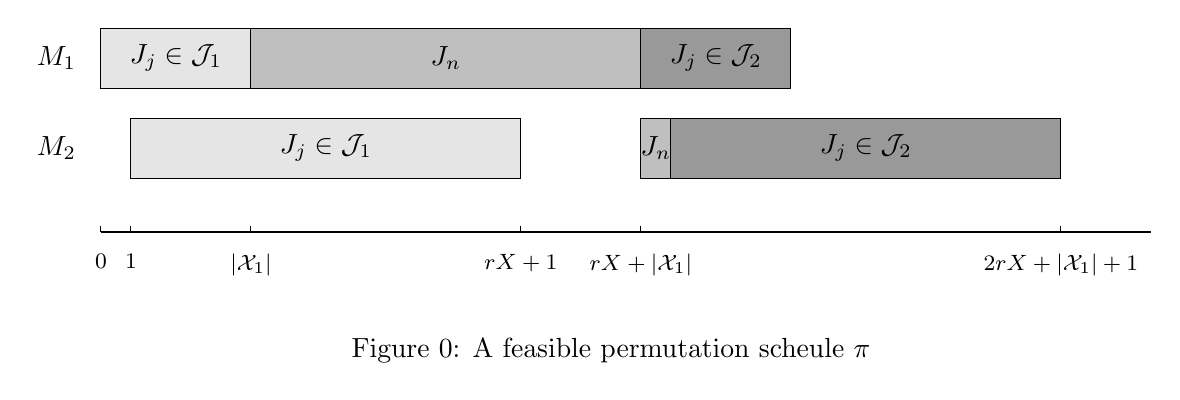
\begin{tikzpicture}[x=0.15in, y=0.3in]

                    \node[anchor=east] at (-0.5,5.5) {$M_1$};
                    \node[anchor=east] at (-0.5,4) {$M_2$};

                    \draw[fill=gray!20] (0,5)   rectangle (5,6)   node[midway] {$J_j \in \mathcal{J}_1$};
                    \draw[fill=gray!50] (5,5)   rectangle (18,6)   node[midway] {$J_n$};
                    \draw[fill=gray!80] (18,5)   rectangle (23,6)  node[midway] {$J_j \in \mathcal{J}_2$};

                    \draw[fill=gray!20] (1,3.5)  rectangle (14,4.5)  node[midway] {$J_j \in \mathcal{J}_1$};
                    \draw[fill=gray!50] (18,3.5)  rectangle (19,4.5) node[midway] {$J_n$};
                    \draw[fill=gray!80] (19,3.5) rectangle (32,4.5)  node[midway] {$J_j \in \mathcal{J}_2$};

                    \draw[thick] (0,2.6) -- (35,2.6);
                    \foreach \x/\label in {0/0, 1/1, 5/$|\mathcal{X}_1|$, 14/$rX+1$, 18/$rX +|\mathcal{X}_1|$, 32/$2rX+|\mathcal{X}_1|+1$}
                    {
                        \draw (\x,2.6) -- (\x,2.7);
                        \node[below, font=\footnotesize] at (\x,2.4) {\label};
                    }

                    % caption
                    \node[below] at (17,1) {Figure~\thefigure: A feasible permutation scheule $\pi$};
                \end{tikzpicture}
                \label{fig:nphard-partition}
            \end{figure}

        Since $a_j \leq b_j$ for each $j=1, 2, \ldots, r$ and $|\mathcal{X}_1| \leq r-1$, it can be easily verified that $C_n(\pi)=rX +|\mathcal{X}_1|+1 \leq r(X+1)$ and $C_{\max}(\pi)=2rX+|\mathcal{X}_1|+1 \leq r(2X+1)$.
        Hence, $C_{\max}^w(\pi) \leq r(X+1)(2X+1)= Y$.

        Conversely, suppose that $F2 \mid \mid C_{\max}^w$ admits a feasible schedule $\pi$ with $C_{\max}^w(\pi) \leq Y$.
        Let $\mathcal{J}_1=\{J_j: C_j(\pi) <C_n(\pi)\}$ and $\mathcal{J}_2=\{J_j: C_j(\pi) > C_n(\pi)\}$ be the sets of jobs completed before and after $J_n$ in $\pi$, respectively, and let $\mathcal{X}_1=\{j: J_j \in \mathcal{J}_1\}$ and $\mathcal{X}_2=\{j: J_j \in \mathcal{J}_2\}$.
        By \cref{eq:completion}, we have
            \begin{equation}\label{eq:completetime1}
                C_n(\pi) \geq \sum_{j \in \mathcal{X}_1} a_j +a_n+ 1=|\mathcal{X}_1| +r X + 1
            \end{equation}
        and
            \begin{equation}\label{eq:completetime2}
                C_n(\pi) \geq a_{\pi(1)}+\sum_{j \in \mathcal{X}_1} b_j+b_n = r \sum_{j \in \mathcal{X}_1} x_j + 2.
            \end{equation}

        \textbf{Case 1.} If $\sum_{j \in \mathcal{X}_1} x_j > X$, then $\sum_{j \in \mathcal{X}_1} x_j \geq X+1$ because the $x_j$ are integers.
        By \cref{eq:completetime2}, $W C_{\max}(\pi) \geq w_n C_n(\pi) \geq (2X+1) (r(X+1)+2) >r(X+1)(2X+1)=Y$, contradicting the assumption that $C_{\max}^w(\pi) \leq Y$.

        \textbf{Case 2.} If $\sum_{j \in \mathcal{X}_1} x_j < X$, then $\sum_{j \in \mathcal{X}_1} x_j \leq X-1$ because the $x_j$ are integers.
        Since $(\mathcal{X}_1, \mathcal{X}_2)$ is a partition of $\{1, 2, \ldots, r\}$, we have
            \begin{equation} \label{eq:sum}
                \sum_{j \in \mathcal{X}_2} x_j =2X-\sum_{j \in \mathcal{X}_1} x_j \geq X+1.
            \end{equation}
        By \cref{eq:completion}, \cref{eq:completetime1}, and \cref{eq:sum}, we have
            \begin{equation}\label{eq:completetime3}
                C_{\pi(n)}(\pi)=C_{\max}(\pi) \geq C_n(\pi)+\sum_{j \in \mathcal{X}_2} b_j \geq |\mathcal{X}_1| +r X + 1+ r \sum_{j \in \mathcal{X}_2} x_j \geq r (2X + 1)+1.
            \end{equation}
        Using $w_{\pi(n)}=1$, \cref{eq:completetime3} yields
            \begin{equation*}
                C_{\max}^w(\pi) \geq w_{\pi(n)} C_{\pi(n)}(\pi) \geq (X+1) (r(2X+1)+1) >r(X+1)(2X+1)=Y,
            \end{equation*}
        This contradicts the assumption that $C_{\max}^w(\pi) \leq Y$.

        Combining the above two cases, we obtain that $\sum_{j \in \mathcal{X}_1} x_j = \sum_{j \in \mathcal{X}_2} x_j= X$.
        Therefore, $(\mathcal{X}_1, \mathcal{X}_2)$ is a solution to \textsc{Partition}.
        \end{proof}

        \begin{theorem}\label{thm:snphard}
        $F2 \mid \mid C_{\max}^w$ is strongly $\mathcal{NP}$-hard when $K$ is arbitrary.
        \end{theorem}
        \begin{proof}
        To establish the result, we give a polynomial-time reduction from 3-\textsc{Partition}, which is strongly  $\mathcal{NP}$-complete \citep{GareyJohnson1979computer}.

        3-\textsc{Partition}: Given $3r$ positive integers $x_1, x_2, \ldots, x_{3r}$ and an integer $X$ with $\sum_{i=1}^{3r}x_i=rX$ and $\frac{X}{4} < x_j < \frac{X}{2}$ for each $j=1, 2, \ldots, 3r$, does there exist a partition of $\{1, 2, \ldots, 3r\}$ into $m$ disjoint subsets $\mathcal{X}_1, \mathcal{X}_2, \ldots, \mathcal{X}_r$ such that $\sum_{j \in \mathcal{X}_i} x_j=X$ for $i=1, 2, \ldots, r$?

        Given an arbitrary instance $(x_1, x_2, \ldots, x_{3r}; X)$ of 3-\textsc{Partition}, we construct an instance of $F2 \mid \mid C_{\max}^w$ consisting of $r$ separating jobs and $3r$ basic jobs.
        For $j=1, 2, \ldots, r$, separating job $J_j$ has $a_j=4X$, $b_j=X$, and $w_j=\frac{5r+4}{5j}$; for $j=r+1, r+2, \ldots, 4r$, basic job $J_j$ has $a_j=x_{j-r}$, $b_j=4 x_{j-r}$, and $w_j=1$.
        Set the threshold to $Y=(5r+4)X$.
        The question is whether there exists a schedule with $W C_{\max} \leq Y$.

        We demonstrate that $F2 \mid \mid C_{\max}^w$ has a feasible schedule $\pi$ with $C_{\max}^w(\pi) \leq Y$ if and only if 3-\textsc{Partition} has a solution.

        Suppose that 3-\textsc{Partition} admits a solution $(\mathcal{X}_1, \mathcal{X}_2, \ldots, \mathcal{X}_r)$, so that $\sum_{j \in \mathcal{X}_i} x_j=X$ and $|\mathcal{X}_i|=3$ for all $i$.
        Let $\mathcal{J}_i=\{J_{r+j}: j \in \mathcal{X}_i\}$ for $i=1, 2, \ldots, r$.
        We build a feasible permutation schedule $\pi$ in which both machines process the jobs in the order
            \begin{equation*}
                J_1 \to \mathcal{J}_1 \to J_2 \to \mathcal{J}_2 \to \cdots \to J_r \to \mathcal{J}_r,
            \end{equation*}
        with the jobs in each $\mathcal{J}_i$ processed in arbitrary order (see \Cref{fig:nphard-3-partition}).

            \begin{figure}[H]
                \centering
                \refstepcounter{figure}
                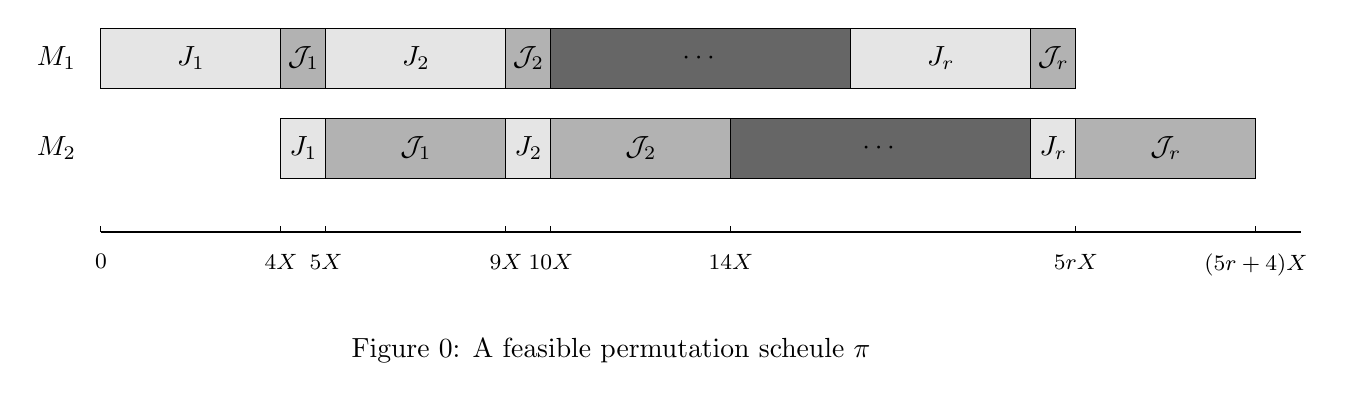
\begin{tikzpicture}[x=0.15in, y=0.3in]

                    \node[anchor=east] at (-0.5,5.5) {$M_1$};
                    \node[anchor=east] at (-0.5,4) {$M_2$};

                    \draw[fill=gray!20] (0,5)   rectangle (6,6)   node[midway] {$J_1$};
                    \draw[fill=gray!60] (6,5)   rectangle (7.5,6)   node[midway] {$\mathcal{J}_1$};
                    \draw[fill=gray!20] (7.5,5)   rectangle (13.5,6)  node[midway] {$J_2$};
                    \draw[fill=gray!60] (13.5,5)   rectangle (15,6)   node[midway] {$\mathcal{J}_2$};
                    \draw[fill=gray!120] (15,5)   rectangle (25,6)   node[midway] {$\cdots$};
                    \draw[fill=gray!20] (25,5)   rectangle (31,6)   node[midway] {$J_{r}$};
                    \draw[fill=gray!60] (31,5)   rectangle (32.5,6)   node[midway] {$\mathcal{J}_r$};

                    \draw[fill=gray!20] (6,3.5)  rectangle (7.5,4.5)  node[midway] {$J_1$};
                    \draw[fill=gray!60] (7.5,3.5)  rectangle (13.5,4.5) node[midway] {$\mathcal{J}_1$};
                    \draw[fill=gray!20] (13.5,3.5) rectangle (15,4.5)  node[midway] {$J_2$};
                    \draw[fill=gray!60] (15,3.5)  rectangle (21,4.5) node[midway] {$\mathcal{J}_2$};
                    \draw[fill=gray!120] (21,3.5)  rectangle (31,4.5) node[midway] {$\cdots$};
                    \draw[fill=gray!20] (31,3.5) rectangle (32.5,4.5)  node[midway] {$J_r$};
                    \draw[fill=gray!60] (32.5,3.5)  rectangle (38.5,4.5) node[midway] {$\mathcal{J}_r$};

                    \draw[thick] (0,2.6) -- (40,2.6);
                    \foreach \x/\label in {0/0, 6/$4X$, 7.5/$5X$, 13.5/$9X$, 15/$10X$, 21/$14X$, 32.5/$5rX$, 38.5/$(5r+4)X$}
                    {
                        \draw (\x,2.6) -- (\x,2.7);
                        \node[below, font=\footnotesize] at (\x,2.4) {\label};
                    }

                    % caption
                    \node[below] at (17,1) {Figure~\thefigure: A feasible permutation scheule $\pi$};
                \end{tikzpicture}
                \label{fig:nphard-3-partition}
            \end{figure}

        According to \Cref{fig:nphard-3-partition}, it can be easily verified that $C_j(\pi)=5jX$ for $j=1, 2, \ldots, r$, and $C_j(\pi) \leq C_{\max}(\pi)=(5r+4)X$ for $j=r+1, r+2, \ldots, 4r$.
        Then $w_j C_j(\pi)=(5r+4)X=Y$ for $j=1, 2, \ldots, r$, and $w_j C_j(\pi) \leq w_j C_{\max}(\pi)=(5r+4)X=Y$ for $j=r+1, r+2, \ldots, 4r$.
        Hence, $C_{\max}^w(\pi) \leq Y$.

        Conversely, suppose that $F2 \mid \mid C_{\max}^w$ admits a feasible schedule $\pi$ with $C_{\max}^w(\pi) \leq Y$.
        Because all separating jobs have the same processing time on $M_1$ and $M_2$ and weights $w_1 >w_2 > \cdots > w_r$, a standard interchange argument lets us assume they appear in $\pi$ in decreasing order of weight.

        \textbf{Claim 1.} $C_{\max}(\pi) \leq Y=(5r+4)X$.

        \textit{Proof of Claim 1.}  Since $w_j \geq 1$ for all $1 \leq j \leq 4r$, we have $C_{\max}(\pi) \leq C_{\max}^w(\pi) \leq Y=(5r+4)X$.
        \hfill$\blacksquare$

        \textbf{Claim 2.} $J_1$ is the first job scheduled in $\pi$.

        \textit{Proof of Claim 2.}  Since $C_{\max}^w(\pi) \leq Y=(5r+4)X$ and $w_1=\frac{5r+4}{5}$, we have $a_1+b_1 \leq C_1(\pi) \leq \frac{C_{\max}^w(\pi)}{w_1} \leq 5X=a_1+b_1$.
        This means that $J_1$ is the first job scheduled in $\pi$.
        \hfill$\blacksquare$

        For $i=1, 2, \ldots, r-1$, let $\mathcal{B}_i=\{J_j: C_i(\pi) < C_j(\pi) < C_{i+1}(\pi)\}$ be the set of basic jobs scheduled between $J_i$ and $J_{i+1}$ in $\pi$, and let $\mathcal{B}_r=\{J_j: C_j(\pi) > C_r(\pi)\}$ be the set of basic jobs scheduled after $J_r$.
        For $i=1, 2, \ldots, r$, define $\mathcal{X}_i=\{j-r: J_j \in  \mathcal{B}_i\}$.
        Then, by Claim 2, $\pi$ can be written as
            \begin{equation} \label{eq:order}
                \pi=(J_1 \to \mathcal{B}_1 \to J_2 \to \mathcal{B}_2 \to \cdots \to J_r \to \mathcal{B}_r).
            \end{equation}

        Since $(\mathcal{X}_1, \mathcal{X}_2, \ldots, \mathcal{X}_r)$ is a partition of $\{1, 2, \ldots, 3r\}$, we have
            \begin{equation} \label{eq:00}
                \sum_{i=1}^r \sum_{j \in \mathcal{X}_i} x_j =\sum_{j=1}^{3r} x_j =rX.
            \end{equation}

        \textbf{Claim 3.} For $k=1, 2, \ldots, r-1$, $\sum_{i=1}^k \sum_{j \in \mathcal{X}_i} x_j \leq kX$.

        \textit{Proof of Claim 3.} Suppose to the contrary that there exists some $m$ ($1 \leq m \leq r-1$) with $\sum_{i=1}^m \sum_{j \in \mathcal{X}_i} x_j > mX$.
        Since the $x_j$ are integers, this implies
            \begin{equation}\label{eq:10}
                \sum_{i=1}^m \sum_{j \in \mathcal{X}_i} x_j \geq mX+1.
            \end{equation}
        Because $a_j=4X$ and $b_j=X$ for $1 \leq j \leq r$, and $a_j=x_{j-r}$ for $r+1 \leq j \leq 4r$, \cref{eq:completion}, \cref{eq:order}, and \cref{eq:10} give
            \begin{equation} \label{eq:11}
                C_{m+1}(\pi) \geq \sum_{j=1}^{m+1} a_j+\sum_{i=1}^m \sum_{j \in \mathcal{B}_i} a_j+b_{m+1} =4(m+1)X+\sum_{i=1}^m \sum_{j \in \mathcal{X}_i} x_j +X \geq 5(m+1)X+1.
            \end{equation}
        Using $w_{m+1}=\frac{5r+4}{5(m+1)}$, \cref{eq:11} yields
            \begin{equation} \label{eq:12}
                C_{\max}^w(\pi) \geq w_{m+1} C_{m+1}(\pi) \geq \frac{5r+4}{5(m+1)} (5(m+1)X+1)>(5r+4)X=Y,
            \end{equation}
        which contradicts the assumption that $C_{\max}^w(\pi) \leq Y$.
        Hence, Claim 3 holds.
        \hfill$\blacksquare$

        \textbf{Claim 4.} For $k=1, 2, \ldots, r-1$, $\sum_{i=1}^k \sum_{j \in \mathcal{X}_i} x_j \geq kX$.

        \textit{Proof of Claim 4.} Suppose to the contrary that there exists some $m$ ($1 \leq m \leq r-1$) with $\sum_{i=1}^m \sum_{j \in \mathcal{X}_i} x_j < mX$.
        By \cref{eq:00} and the $x_j$ are integers, we have
            \begin{equation}\label{eq:20}
                \sum_{i=m+1}^r \sum_{j \in \mathcal{X}_i} x_j=rX-\sum_{i=1}^m \sum_{j \in \mathcal{X}_i} x_j \geq (r-m)X+1.
            \end{equation}
        Because $a_j=4X$ and $b_j=X$ for $1 \leq j \leq r$, and $a_j=x_{j-r}$ and $b_j=4 x_{j-r}$ for $r+1 \leq j \leq 4r$, \cref{eq:completion}, \cref{eq:order}, \cref{eq:00}, and \cref{eq:20} give
            \begin{align*}
                C_{\max}(\pi) & \geq \sum_{j=1}^{m+1} a_j+\sum_{i=1}^m \sum_{j \in \mathcal{B}_i} a_j+\sum_{j=m+1}^r      b_j+\sum_{i=m+1}^r \sum_{j \in \mathcal{B}_i} b_j  \nonumber \\
                &= 4(m+1)X+\sum_{i=1}^m \sum_{j \in \mathcal{X}_i} x_j +(r-m)X +\sum_{i=m+1}^r \sum_{j \in \mathcal{X}_i} 4 x_j \nonumber \\
                &= 4(m+1)X +(r-m)X + rX+ 3 \sum_{i=m+1}^r \sum_{j \in \mathcal{X}_i} x_j \\
                & \geq 4(m+1)X +(r-m)X + rX+ 3((r-m)X+1)  \nonumber \\
                & = (5r+4)X +3 > (5r+4)X = Y. \nonumber
            \end{align*}
        which contradicts Claim 1.
        Hence, Claim 4 holds.
        \hfill$\blacksquare$

        Combining Claims 3 and 4 with \cref{eq:00}, we obtain that $\sum_{j \in \mathcal{X}_i} x_j=X$ for $i=1, 2, \ldots, r$.
        Since $X/4 < x_j < X/2$ for each $j$, a sum equal to $X$ must contain exactly three elements; hence  $|\mathcal{X}_i|=3$ for each $i$.
        Therefore, $(\mathcal{X}_1, \mathcal{X}_2, \ldots, \mathcal{X}_r)$ is a solution to 3-\textsc{Partition}.
        \end{proof}

        \section{Fixed number of weights} \label{sec:dp_algorithm}

        In this section, we focus on the case where the number of weights $K$ is fixed, i.e., $K=O(1)$.
        For $K=1$, the problem is exactly $F2 \mid \mid C_{\max}$, which Johnson's rule solves in $O(n \log n)$ time \citep{Johnson1954NRL}; the rule is summarized in \Cref{alg:Johnson}.
        For $K=2$, the problem $F2 \mid \mid C_{\max}^w$ is already binary $\mathcal{NP}$-hard (\Cref{thm:nphard}).
        For fixed $K$, we develop an exact DP algorithm running in pseudo-polynomial time and derive an FPTAS from it.

        \begin{algorithm}[H]
            \small
            \SetAlgoLined
            \DontPrintSemicolon
            \caption{Johnson's rule for $F2\mid\mid C_{\max}$}\label{alg:Johnson}
            \KwIn{Job set $\mathcal{J}$; job parameters $a_j$ and $b_j$ for $j=1, 2, \ldots, n$.}
            \BlankLine
            \textbf{Step 1.} Partition $\mathcal{J}$ into two sets $\mathcal{J}^1=\{J_j: a_j \leq b_j\}$
            and $\mathcal{J}^2=\{J_j: a_j>b_j\}$.

            \textbf{Step 2.} Order the jobs in $\mathcal{J}^1$ in nondecreasing order of $a_j$, followed by those in $\mathcal{J}^2$ in nondecreasing order of $b_j$. \;

            \textbf{Step 3.} Process the jobs in this order on $M_1$ and then on $M_2$, yielding the permutation schedule $\pi$. \;

            \KwOut{The resulting schedule $\pi$.}
        \end{algorithm}

        Let $W_1 > W_2 > \cdots > W_K$ denote the distinct weights of the $n$ jobs, and let $\mathcal{G}_k = \{J_j \in \mathcal{J}: w_j = W_k\}$ be set of jobs having weight $W_k$, $k=1, 2,\ldots, K$.

        \subsection{Block structure of an optimal schedule} \label{sec:block}

        To establish the key structural lemma, we first introduce some notation for partitioning a permutation schedule into blocks.
        \begin{definition} \label{def:block}
        \textbf{(Block partition)} Let $\pi = (\pi(1), \pi(2), \ldots, \pi(n))$ be a permutation schedule.
        Set $\ell_0 = 0$ and $\mathcal{R}_1=\mathcal{J}$.
        For $k = 1, 2, \ldots, K$, if $\mathcal{R}_k \cap \mathcal{G}_k \neq \emptyset$, define $\ell_k=\max \{j: J_{\pi(j)} \in \mathcal{R}_k \cap \mathcal{G}_k\}$, $\mathcal{B}_k^{\pi} = \{J_{\pi(\ell_{k-1}+1)}, J_{\pi(\ell_{k-1}+2)}, \ldots, J_{\pi(\ell_k)}\}$, and $\mathcal{R}_{k+1}=\mathcal{J}\setminus\bigcup_{i=1}^{k}\mathcal{B}_i^{\pi}$.
        Otherwise, set $\ell_k=\ell_{k-1}$,  $\mathcal{B}_k^{\pi} =\emptyset$, and $\mathcal{R}_{k+1}=\mathcal{R}_{k}$.
        Then we call $\mathcal{B}(\pi)=(\mathcal{B}_1^{\pi}, \mathcal{B}_2^{\pi}, \ldots, \mathcal{B}_K^{\pi})$ the block partition of $\pi$.
        \end{definition}

        Thus, $\ell_k$ is the position of the last job in $\mathcal{R}_k$ of weight $W_k$, $\mathcal{B}_k^{\pi}$ is the $k$-th block (possibly empty), and $\mathcal{R}_k$ is the set of jobs left after removing the first $k-1$ blocks.
        By construction, every nonempty block $\mathcal{B}_k^{\pi}$ ends with a job of weight $W_k$ (i.e., $w_{\pi(\ell_k)}=W_k$), and all jobs in the block have weight at most $W_k$, i.e., $w_{\pi(j)} \leq W_k$ for all  $\ell_{k-1}+1 \leq j \leq \ell_{k}$.
        This means that
        \begin{equation} \label{eq:block-1}
            W_k C_{\pi(\ell_k)}(\pi)=\max \{w_{\pi(j)} C_{\pi(j)}(\pi): \ell_{k-1}+1 \leq j \leq \ell_{k}\}.
        \end{equation}
        Consequently, \cref{eq:wcmax} can be reformulated as
        \begin{equation}\label{eq:block-comp}
            C_{\max}^w(\pi)=\max_{1 \leq k \leq K} \{W_k C_{\pi(\ell_k)(\pi)}\}.
        \end{equation}

        \begin{definition}\label{def:regular}
        \textbf{(Regular block and regular permutation schedule)} Let $\pi=(\pi(1),\pi(2),\ldots,\pi(n))$ be a permutation schedule with block partition $\mathcal{B}(\pi)=(\mathcal{B}_1^{\pi},\mathcal{B}_2^{\pi},\ldots,\mathcal{B}_K^{\pi})$.
        A block $\mathcal{B}_k^{\pi}$ is called regular if it is empty or if the sequence of its jobs in $\pi$ matches the sequence obtained by applying Johnson's rule to that block.
        The schedule $\pi$ is called regular if all blocks  $\mathcal{B}_1^{\pi},\mathcal{B}_2^{\pi},\ldots,\mathcal{B}_K^{\pi}$ are regular.
        \end{definition}

        To illustrate the block partition, we give a small numerical example for $F2 \mid \mid C_{\max}^w$.

        \begin{exam}\label{ex:blocking}
            Consider a six-job instance of $F2 \mid \mid C_{\max}^w$ whose job data are given in \Cref{tab:TA-2-1}, and let $\pi = (1, 2, \ldots, 6)$ be a permutation schedule.
        \end{exam}
        \begin{table}[htbp]
            \small
            \centering
            \caption{Job data for \Cref{ex:blocking}}   \label{tab:TA-2-1}
            \begin{tabular}{c|cccccc}
                & $J_1$ & $J_2$ & $J_3$ & $J_4$ & $J_5$ & $J_6$ \\
                \hline
                $a_j$ & 2 & 5 & 6 & 8 & 2 & 3 \\
                $b_j$ & 5 & 3 & 9 & 4 & 3 & 3 \\
                $w_j$ & 2 & 3 & 5 & 2 & 3 & 2 \\
            \end{tabular}
        \end{table}

        In \Cref{ex:blocking}, we have $K=3$, $\mathcal{G}_1=\{J_3\}$, $\mathcal{G}_2=\{J_2, J_5\}$, and $\mathcal{G}_3=\{J_1,J_4,J_6\}$.
        The resulting blocks are $\mathcal{B}_1^{\pi}=\{J_1,J_2,J_3\}$, $\mathcal{B}_2^{\pi}=\{J_4,J_5\}$, and $\mathcal{B}_3^{\pi}=\{J_6\}$ (see \Cref{fig:exam}).
        By \cref{eq:block-comp}, the weighted makespan of $\pi$ is $C_{\max}^w(\pi)=\max \{5 \times 22, 3 \times 29, 2 \times 32\}=110$.

        \begin{figure}[H]
            \centering
            \refstepcounter{figure}
            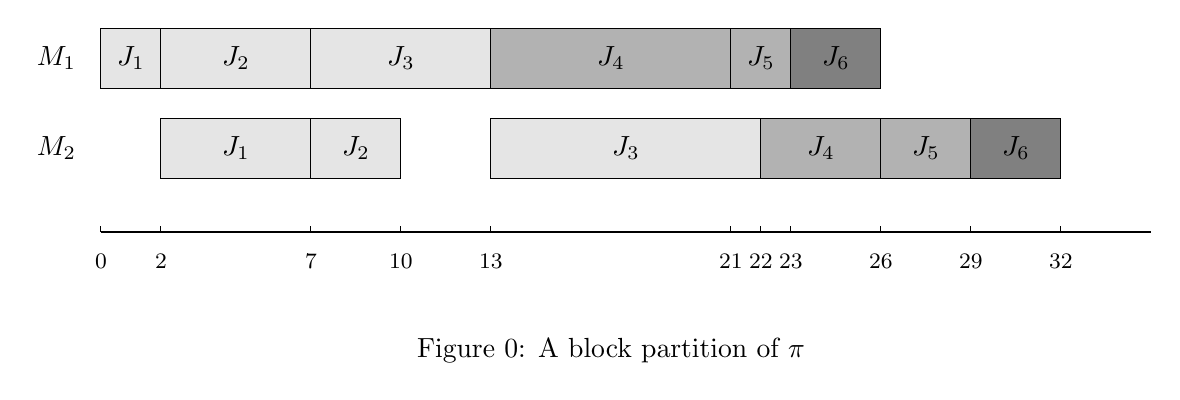
\begin{tikzpicture}[x=0.15in, y=0.3in]
                % machine index
                \node[anchor=east] at (-0.5,5.5) {$M_1$};
                \node[anchor=east] at (-0.5,4) {$M_2$};

                \draw[fill=gray!20] (0,5)   rectangle (2,6)   node[midway] {$J_1$};
                \draw[fill=gray!20] (2,5)   rectangle (7,6)   node[midway] {$J_2$};
                \draw[fill=gray!20] (7,5)   rectangle (13,6)  node[midway] {$J_3$};
                \draw[fill=gray!60] (13,5)  rectangle (21,6)  node[midway] {$J_4$};
                \draw[fill=gray!60] (21,5)  rectangle (23,6)  node[midway] {$J_5$};
                \draw[fill=gray!100] (23,5)  rectangle (26,6)  node[midway] {$J_6$};

                \draw[fill=gray!20] (2,3.5)  rectangle (7,4.5)  node[midway] {$J_1$};
                \draw[fill=gray!20] (7,3.5)  rectangle (10,4.5) node[midway] {$J_2$};
                \draw[fill=gray!20] (13,3.5) rectangle (22,4.5) node[midway] {$J_3$};
                \draw[fill=gray!60] (22,3.5) rectangle (26,4.5) node[midway] {$J_4$};
                \draw[fill=gray!60] (26,3.5) rectangle (29,4.5) node[midway] {$J_5$};
                \draw[fill=gray!100] (29,3.5) rectangle (32,4.5) node[midway] {$J_6$};

                % x-axis
                \draw[thick] (0,2.6) -- (35,2.6);
                \foreach \x/\label in {0/0, 2/2, 7/7, 10/10, 13/13, 21/21, 22/22, 23/23, 26/26, 29/29, 32/32} {
                    \draw (\x,2.6) -- (\x,2.7);
                    \node[below, font=\footnotesize] at (\x,2.4) {\label};
                }

                % caption
                \node[below] at (17,1) {Figure~\thefigure: A block partition of $\pi$};    \label{fig:exam}
            \end{tikzpicture}
        \end{figure}

        Given a permutation schedule $\pi=(\pi(1), \pi(2), \ldots, \pi(n))$, for $1 \leq g \leq h \leq n$, define \begin{equation*}
            C_{\max}^w(\pi)[g:h]= \max_{g \leq j \leq h}\{w_{\pi(j)}C_{\pi(j)}(\pi)\}
        \end{equation*}
        as the maximum weighted completion time over the jobs $J_{\pi(g)}, J_{\pi(g+1)}, \ldots, J_{\pi(h)}$.

        The following lemma shows that if the jobs in each block of $\pi$ are rescheduled in accordance with Johnson's rule, the resulting permutation schedule $\pi'$ has objective value no larger than that of $\pi$, i.e., $C_{\max}^w(\pi') \leq C_{\max}^w(\pi)$.

        \begin{lemma}\label{lem:block-johnson}
        Given a permutation schedule $\pi$ and its block partition $\mathcal{B}(\pi)=(\mathcal{B}_1^{\pi}, \mathcal{B}_2^{\pi}, \ldots, \mathcal{B}_K^{\pi})$, let $\pi_k$ be the permutation of $\mathcal{B}_k^{\pi}$ obtained by Johnson's rule for $k=1, 2, \ldots, K$.
        Then the schedule $\pi'$ formed by concatenating $\pi_1, \pi_2, \ldots, \pi_K$ satisfies  $C_{\max}^w(\pi') \leq C_{\max}^w(\pi)$.
        \end{lemma}

        \begin{proof}
        First, if $\mathcal{B}_k^{\pi} \neq \emptyset$, then rescheduling the jobs in $\mathcal{B}_k^{\pi}$ according to Johnson's rule does not change the set of jobs assigned to positions $\ell_{k-1}+1, \ell_{k-1}+2, \ldots, \ell_k$, i.e.,
            \begin{equation} \label{eq:induc-1}
                \mathcal{B}_k^{\pi} = \{J_{\pi(\ell_{k-1}+1)}, J_{\pi(\ell_{k-1}+2)}, \ldots, J_{\pi(\ell_k)}\}=\{J_{\pi'(\ell_{k-1}+1)}, J_{\pi'(\ell_{k-1}+2)}, \ldots, J_{\pi'(\ell_k)}\}.
            \end{equation}
        Thus, in $\pi'$, the jobs in $\mathcal{B}_k^{\pi}$ still occupy this same index interval.
        By \cref{eq:block-1}, we have
            \begin{equation}  \label{eq:induc-2}
                C_{\max}^w(\pi)[\ell_{k-1}+1:\ell_k]=W_k C_{\pi(\ell_k)}(\pi)=w_{\pi(\ell_k)} C_{\pi(\ell_k)}(\pi), k=1, 2, \ldots, K.
            \end{equation}
        Moreover, by \cref{eq:induc-1}, for $k=1, 2, \ldots, K$, $\mathcal{B}_k^{\pi}$ has the same completion time on $M_1$ under $\pi$ and $\pi'$, i.e., $C_{\pi'(\ell_k)}^1(\pi')=C_{\pi(\ell_k)}^1(\pi)=\sum_{j=1}^{\ell_k} a_{\pi(j)}$.

        Second, we prove by induction on $k$ that, for all $k=1, 2, \ldots, K$,
            \begin{equation} \label{eq:induc-assump}
                C_{\pi'(\ell_k)} (\pi') \leq C_{\pi(\ell_k)}(\pi) ~ \mathrm{and}  ~ C_{\max}^w(\pi')[\ell_{k-1}+1:\ell_k] \leq C_{\max}^w(\pi)[\ell_{k-1}+1:\ell_k].
            \end{equation}

        For the base case $i=1$, both machines are available at time zero.
        Rescheduling the jobs in $\mathcal{B}_1^{\pi}$ according to Johnson's rule gives $C_{\pi'(\ell_1)}(\pi') \leq C_{\pi(\ell_1)}(\pi)$.
        Since $\pi'$ only permutes the jobs in $\mathcal{B}_1^{\pi}$, we have $w_{\pi'(j)} \leq W_1$ for $j=1, 2, \ldots, \ell_1$.
        Hence, we have
            \begin{equation*}
                C_{\max}^w(\pi')[1:\ell_1]= \max_{1 \leq j \leq \ell_1}\{w_{\pi'(j)}C_{\pi'(j)}(\pi')\} \leq W_1 C_{\pi'(\ell_1)}(\pi') \leq W_1 C_{\pi(\ell_1)}(\pi)=C_{\max}^w(\pi)[1:\ell_1],
            \end{equation*}
        where the last equality follows from \cref{eq:induc-2}

        Assume that \cref{eq:induc-assump} holds for all $i=1, 2, \ldots, k$.
        We now prove the $(k+1)$-block.
        If $\mathcal{B}_{k+1}^{\pi}=\emptyset$, the assertion is immediate.
        It remains to consider $\mathcal{B}_{k+1}^{\pi} \neq \emptyset$.
        In this case, in $\pi'$, by the inductive hypothesis, $M_1$ becomes available at time $C_{\pi'(\ell_k)}^1(\pi')=C_{\pi(\ell_k)}^1(\pi)$, and $M_2$ is available at time $C_{\pi'(\ell_k)}(\pi') \leq C_{\pi(\ell_k)}(\pi)$.
        We introduce a dummy job $J_0$ with processing times $a_0=0$ and $b_0=C_{\pi'(\ell_k)}(\pi')-C_{\pi'(\ell_k)}^1(\pi')$, and apply Johnson's rule to schedule the jobs in $\mathcal{B}_{k+1}^{\pi} \cup \{J_0\}$, with both machines available from time $C_{\pi'(\ell_k)}^1(\pi')$.
        Because $a_0=0$, $J_0$ is scheduled in the first position according to Johnson's rule, and it completes at time $C_{\pi'(\ell_k)}(\pi')$.
        By positioning the dummy job in this way, the jobs in $\mathcal{B}_{k+1}^{\pi}$ can be scheduled on $M_2$ without overlapping with the previously scheduled jobs in $\mathcal{B}_1^{\pi} \cup \mathcal{B}_2^{\pi} \cup \cdots \cup \mathcal{B}_k^{\pi}$.
        Since the jobs in $\mathcal{B}_{k+1}$ are scheduled according to Johnson's rule, it follows that $C_{\pi'(\ell_{k+1})} (\pi') \leq C_{\pi(\ell_{k+1})}(\pi)$.
        Moreover, since $\pi'$ only permutes the jobs in $\mathcal{B}_{k+1}^{\pi}$, we have $w_{\pi'(j)} \leq W_{k+1}$ for $j=\ell_k+1, \ell_k+2, \ldots, \ell_{k+1}$.
        Hence,
            \begin{align*}
                C_{\max}^w(\pi')[\ell_k+1:\ell_{k+1}] & = \max_{\ell_k+1 \leq j \leq \ell_{k+1}}\{w_{\pi'(j)}C_{\pi'(j)}(\pi')\} \leq W_{k+1} C_{\pi'(\ell_{k+1})}(\pi') \\
                & \leq W_{k+1} C_{\pi(\ell_{k+1})}(\pi)=C_{\max}^w(\pi)[\ell_k+1:\ell_{k+1}],
            \end{align*}
        where the last equality follows from \cref{eq:induc-2}.
        This completes the inductive step.

        Note that $C_{\max}^w(\pi')=\max\limits_{1 \leq k \leq K} \{C_{\max}^w(\pi')[\ell_{k-1}+1:\ell_k]\}$ and $C_{\max}^w(\pi)=\max\limits_{1 \leq k \leq K} \{C_{\max}^w(\pi)[\ell_{k-1}+1:\ell_k]\}$.
        Hence, \cref{eq:induc-assump} yields $C_{\max}^w(\pi') \leq C_{\max}^w(\pi)$.
        \end{proof}

        To illustrate \Cref{lem:block-johnson}, consider \Cref{ex:blocking}.
        Given $\pi$ and its block partition $\mathcal{B}(\pi)=(\mathcal{B}_1^{\pi}, \mathcal{B}_2^{\pi}, \mathcal{B}_3^{\pi})$, we apply Johnson’s rule independently within each block $\mathcal{B}_k^{\pi}$, $k=1, 2, 3$, obtaining a permutation $\pi_k$ of the jobs in that block.
        Concatenating $\pi_1, \pi_2, \pi_3$ gives $\pi'=(1, 3, 2, 5, 4, 6)$, with blocks $\mathcal{B}_1^{\pi'}=\{J_1,J_3\}$, $\mathcal{B}_2^{\pi'}=\{J_2,J_5\}$, and $\mathcal{B}_3^{\pi'}=\{J_4, J_6\}$ (see \Cref{fig:exam-2}).
        By \cref{eq:block-comp}, the weighted makespan of $\pi'$ is $C_{\max}^w(\pi')=\max \{5 \times 17, 3 \times 23, 2 \times 30\}=85$.

        \begin{figure}[H]
            \centering
            \refstepcounter{figure}
            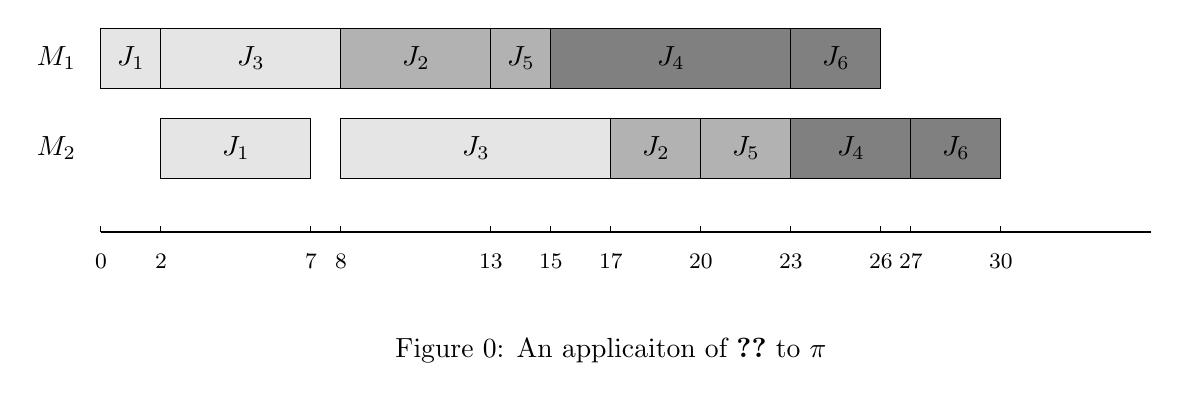
\begin{tikzpicture}[x=0.15in, y=0.3in]
                % machine index
                \node[anchor=east] at (-0.5,5.5) {$M_1$};
                \node[anchor=east] at (-0.5,4) {$M_2$};

                \draw[fill=gray!20] (0,5)   rectangle (2,6)   node[midway] {$J_1$};
                \draw[fill=gray!20] (2,5)   rectangle (8,6)   node[midway] {$J_3$};
                \draw[fill=gray!60] (8,5)   rectangle (13,6)  node[midway] {$J_2$};
                \draw[fill=gray!60] (13,5)  rectangle (15,6)  node[midway] {$J_5$};
                \draw[fill=gray!100] (15,5)  rectangle (23,6)  node[midway] {$J_4$};
                \draw[fill=gray!100] (23,5)  rectangle (26,6)  node[midway] {$J_6$};

                \draw[fill=gray!20] (2,3.5)  rectangle (7,4.5)  node[midway] {$J_1$};
                \draw[fill=gray!20] (8,3.5)  rectangle (17,4.5) node[midway] {$J_3$};
                \draw[fill=gray!60] (17,3.5) rectangle (20,4.5) node[midway] {$J_2$};
                \draw[fill=gray!60] (20,3.5) rectangle (23,4.5) node[midway] {$J_5$};
                \draw[fill=gray!100] (23,3.5) rectangle (27,4.5) node[midway] {$J_4$};
                \draw[fill=gray!100] (27,3.5) rectangle (30,4.5) node[midway] {$J_6$};

                % x-axis
                \draw[thick] (0,2.6) -- (35,2.6);
                \foreach \x/\label in {0/0, 2/2, 7/7, 8/8, 13/13, 15/15, 17/17, 20/20, 23/23, 26/26, 27/27, 30/30} {
                    \draw (\x,2.6) -- (\x,2.7);
                    \node[below, font=\footnotesize] at (\x,2.4) {\label};
                }

                % caption
                \node[below] at (17,1) {Figure~\thefigure: An applicaiton of \Cref{lem:block-johnson} to $\pi$};    \label{fig:exam-2}
            \end{tikzpicture}
        \end{figure}

        \begin{lemma}\label{lem:regular-schedule}
        For $F2 \mid \mid C_{\max}^w$, there exists an optimal permutation schedule that is regular.
        \end{lemma}

        \begin{proof}
        Let $\pi$ be an optimal permutation schedule for $F2 \mid \mid C_{\max}^w$.
        If $\pi$ is regular, the lemma follows.
        Otherwise, let $\mathcal{B}(\pi)=(\mathcal{B}_1^{\pi}, \mathcal{B}_2^{\pi}, \ldots, \mathcal{B}_K^{\pi})$ be its block partition.
        Apply Johnson’s rule within each block $\mathcal{B}_k^{\pi}$ ($k=1, 2, \ldots, K$) to obtain a permutation $\pi_k$, and concatenate $\pi_1, \pi_2, \ldots, \pi_K$ to form a permutation schedule $\pi'$.
        By \Cref{lem:block-johnson}, $C_{\max}^w(\pi') \leq C_{\max}^w(\pi)$.
        Since $\pi$ is optimal, $\pi'$ is optimal as well.

        If $\pi'$ is regular, the lemma follows.
        Otherwise, repeat the above procedure with $\pi'$ in place of $\pi$.
        For termination, suppose the first $i$ blocks of the current schedule are already regular (initially $i=0$).
        By definition, applying Johnson's rule to a regular block leaves its job sequence unchanged.
        Hence, the first $i$ blocks remain unchanged.
        The $(i+1)$-th block in the resulting schedule may contain a different job set, but it satisfies Johnson's rule.
        Thus the first $i+1$ blocks are regular, so every application increases the number of leading regular blocks by at least one.
        Since there are at most $K$ nonempty blocks in each schedule, the procedure terminates after at most $K$ iterations and yields an optimal regular schedule.
        \end{proof}

        Let $\pi$ be a regular permutation schedule for $F2 \mid \mid C_{\max}^w$ with block partition $\mathcal{B}(\pi)=(\mathcal{B}_1^{\pi}, \mathcal{B}_2^{\pi}, \ldots, \mathcal{B}_K^{\pi})$.
        For each $k=1, 2, \ldots, K$, let $\pi_k$ denote the schedule obtained by processing the jobs in $\mathcal{B}_k^{\pi}$ consecutively from time zero in accordance with Johnson’s rule.
        Note that $\pi$ coincides with the schedule obtained by concatenating $\pi_1, \pi_2, \ldots, \pi_K$.
        This representation allows us to compute $C_{\max}(\pi)$ and $C_{\max}^w(\pi)$ from parameters defined for each $\pi_k$.
        Specifically, for each $k$, let $A_k=A(\pi_k)$ and $B_k=B(\pi_k)$ denote the total processing times of the jobs in $\pi_k$ on $M_1$ and $M_2$, respectively, and let $C_k=C(\pi_k)$ denote the makespan of $\pi_k$.
        Given these parameters, we describe an procedure for computing $C_{\max}(\pi)$ and $C_{\max}^w(\pi)$.
        The procedure starts with $\pi_1$ and successively appends $\pi_2, \pi_3, \ldots, \pi_K$ in that order.
        For $k=1, 2, \ldots, K$, let $\pi[1:k]$ denote the schedule obtained by concatenating $\pi_1, \pi_2, \ldots, \pi_k$; thus $\pi=\pi[1:K]$.
        The makespan and weighted makespan of $\pi[1: k]$ are computed recursively.
        For convenience, set $C_{\max}(\pi[1: 0])=C_{\max}^w(\pi[1: 0])=0$.
        For $k=1, 2, \ldots, K$, by direct calculation and induction on $k$, we have
        \begin{equation}
            \begin{aligned} \label{eq-4.2:block-makespan}
                C_{\max}(\pi[1: k]) &=\max \Big\{\sum_{i=1}^{k-1} A_i+C_k, C_{\max}(\pi[1: k-1])+B_k\Big\}  \\
                &= \max_{0 \leq h \leq k-1} \Big\{ \sum_{i=1}^h A_i +C_{h+1} + \sum_{i=h+2}^k B_i \Big\}
            \end{aligned}
        \end{equation}
        and
        \begin{equation}\label{eq-4.2:block-weighted makespan}
            \begin{aligned}
                C_{\max}^w(\pi[1: k]) &=\max \{C_{\max}^w(\pi[1: k-1]), W_k C_{\max}(\pi[1: k])\}  \\
                &= \max_{1 \leq h \leq k} \{W_h C_{\max}(\pi[1: h])\}.
            \end{aligned}
        \end{equation}
        Hence, $C_{\max}^w(\pi)=C_{\max}^w(\pi[1: K])$.

        \subsection{An exact DP algorithm} \label{sec:dp}

        Recall that $W_1 >W_2 > \cdots W_K$.
        For each job $J_j$ ($j=1, 2, \ldots, n$), let $g_j \in \{1, 2, \ldots, K\}$ be the index such that $w_j=W_{g_j}$, i.e., $J_j\in\mathcal{G}_{g_j}$.
        Assume that the jobs in $\mathcal{J}$ are indexed in accordance with Johnson's rule.

        Building on the preceding discussion in \Cref{sec:block}, we develop an exact DP algorithm for $F2 \mid \mid C_{\max}^w$.
        It generates a sequence of sets $\mathcal{H}_0, \mathcal{H}_1, \ldots, \mathcal{H}_n$.
        Each $\mathcal{H}_j$ consists of $K$-tuples $(X_1, X_2, \ldots, X_K)$, where $X_k=(A_k, B_k, C_k, L_k)$ for $k=1, 2, \ldots, K$.
        A tuple in $\mathcal{H}_j$ ($j=1, 2, \ldots, n$) encodes an assignment of jobs $J_1, J_2, \ldots, J_j$ to $K$ schedules (i.e., blocks) $\pi_1(j), \pi_2(j), \ldots, \pi_K(j)$, with jobs in each schedule processed from time zero in increasing order of their indices.
        For each schedule $\pi_k(j)$, $A_k$ and $B_k$ are the total processing times on $M_1$ and $M_2$, respectively, and $C_k$ and $L_k$ are the makespan of $\pi_k(j)$ and the weight of its last job.

        Initially, $\mathcal{H}_0$ consists of a single tuple, all of whose $4K$ entries are zero, i.e., $\mathcal{H}_0=\{\Big (\underbrace{(0,0,0,0),\ldots,(0,0,0,0)}_{K\text{ copies}}\Big)\}$.
        In the $j$-th iteration ($j=1, 2, \ldots, n$), $\mathcal{H}_j$ is constructed from $\mathcal{H}_{j-1}$.
        For each tuple $(X_1, X_2, \ldots, X_K) \in \mathcal{H}_{j-1}$, with $X_k=(A_k, B_k, C_k, L_k)$ for $k=1, 2, \ldots, K$, the definition of $g_j$ and \Cref{lem:regular-schedule} together imply that this tuple generates $g_j$ new tuples in $\mathcal{H}_j$.
        If $k \leq g_j$, appending $J_j$ to $\pi_k(j-1)$ yields the new tuple $(X_1, \ldots, X_{k-1}, X'_k, X_{k+1}, \ldots, X_K)$ into $\mathcal{H}_j$, where $X'_k=(A'_k, B'_k, C'_k, L'_k)$ is given by
        \begin{equation} \label{eq-4.2: rec}
            A'_k=A_k+a_j, ~ B'_k=B_k+b_j, ~ C'_k=\max\{C_k, A_k + a_j \}+ b_j, ~ L'_k= w_j.
        \end{equation}

        The following lemma will be used to remove dominated tuples during the tuple generation, which can be easily verified.

        \begin{lemma}\label{lem:dominance}
            Let $X=(X_1, X_2, \ldots, X_K)$ and $X'=(X'_1, X'_2, \ldots, X'_K)$ be two tuples
            in $\mathcal{H}_j$, with $X_k=(A_k, B_k, C_k, L_k)$ and $X'_k=(A'_k, B'_k, C'_k, L'_k)$ for $k=1, 2, \ldots, K$. If \begin{equation*}
                A_k = A'_k, ~ B_k = B'_k, ~ C_k=C'_k, ~ L_k = L'_k ~ (k=1, 2, \ldots, K-1),
            \end{equation*}
        $L_K = L'_K$, and $C_K \leq C'_K$, then $X'$ is dominated by $X$ and can therefore be deleted from $\mathcal{H}_j$.
        \end{lemma}

        By \Cref{lem:regular-schedule}, it suffices to consider regular permutation schedules.
        Therefore, once $\mathcal{H}_n$ has been generated, we discard every tuple $(X_1, X_2, \ldots, X_K)$ with $L_k \notin \{0, W_k\}$ for some $k$, since concatenating the schedules corresponding to $X_1, X_2, \ldots, X_K$ cannot yield a regular schedule.
        This does not affect our search for the optimal solution.
        Then, for each retained tuple in $\mathcal{H}_n$, we compute the makespan and weighted makespan according to \cref{eq-4.2:block-makespan} and \cref{eq-4.2:block-weighted makespan}, respectively.

        Summarizing the above analysis and utilizing \Cref{lem:regular-schedule} and \Cref{lem:dominance}, the following algorithm is developed to solve $F2 \mid \mid C_{\max}^w$.

        \begin{algorithm}[H]
            \small
            \linespread{1.2}\selectfont
            \SetAlgoLined
            \DontPrintSemicolon
            \caption{An exact DP algorithm for $F2 \mid \mid C_{\max}^w$} \label{alg:dp}
            \KwIn{Job set $\mathcal{J}$; job parameters $a_j$, $b_j$, $w_j$, and $g_j$ for $j=1, 2, \ldots, n$, $K$ distinct weights with $W_1> W_2 > \cdots > W_K$.}
            \BlankLine
            \textbf{Step 1.} [Preprocessing] Renumber jobs in $\mathcal{J}$ according to Johnson' rule (\Cref{alg:Johnson}). \;

            \textbf{Step 2.} [Initialization] Set $\mathcal{H}_0=\{\Big(\underbrace{(0,0,0,0),\ldots,(0,0,0,0)}_{K\text{ copies}}\Big)\}$, and $\mathcal{H}_j=\emptyset$ for $j=1, 2, \ldots, n$. \;

            \textbf{Step 3.} [Generation of sets $\mathcal{H}_1, \mathcal{H}_2, \ldots, \mathcal{H}_n$]

            \For{$j=1$ \KwTo $n$}
            {
                \For{each $(X_1, X_2, \ldots, X_K) \in \mathcal{H}_{j-1}$ with $X_k=(A_k, B_k, C_k, L_k)$, $k=1, 2, \ldots, K$}
                {
                    \For{$k=1$ \KwTo $g_j$}
                    {
                        $A'_k = A_k+a_j$, $B'_k = B_k+b_j$, $C'_k = \max\{C_{k-1}, A_{k-1}+a_j\}+b_j$, $L'_k= w_j$. \;

                        $X'_k=(A'_k, B'_k, C'_k, L'_k)$. \;

                        Add the tuple $(X_1, \ldots, X_{k-1}, X'_k, X_{k+1}, \ldots, X_K)$ to $\mathcal{H}_j$. \;
                    }
                }
                [Elimination] Among all tuples in $\mathcal{H}_j$ with the same $X_1, X_2, \ldots, X_{K-1}$ and the same $L_K$, retain only the tuple with the smallest $C_K$ (by \Cref{lem:dominance}). \;
            }

            \textbf{Step 4.} [Computation of objective values for the tuples in $\mathcal{H}_n$ ]

            \For{each $X=(X_1, X_2, \ldots, X_K) \in \mathcal{H}_n$ with $X_k=(A_k, B_k, C_k, L_k)$, $k=1, 2, \ldots, K$}
            {
                \eIf{$L_k \in \{0, W_k\}$ for each $k=1, 2, \ldots, K$}
                {
                    Set $T_0^1= 0$, $T_0^2=0$, $Z_0=0$. \;

                    \For{$k=1$ \KwTo $K$}
                    {
                        $T_k^1= T_{k-1}^1+A_k$, $T_k^2 = \max\{T_{k-1}^1+C_k,\ T_{k-1}^2+B_k\}$. \;

                        $Z_k = \max \{Z_{k-1}, L_k \cdot T_k^2\}$. \;
                    }

                    $C_{\max}^w(X)=Z_K$. \;
                }{
                    $C_{\max}^w(X)=+\infty$. \;
                }
            }
            \textbf{Step 5.} [Result] Compute $C_{\max}^w(X_{\mathrm{opt}})=\min \{C_{\max}^w(X): X \in \mathcal{H}_n\}$ and recover the corresponding optimal schedule $\pi_{\mathrm{opt}}$ from $X_{\mathrm{opt}}$ by backtracking. \;

            \KwOut{The optimal schedule $\pi_{\mathrm{opt}}$.}
        \end{algorithm}


        \begin{theorem}\label{thm:complexity}
        \Cref{alg:dp} solves $F2 \mid \mid C_{\max}^w$ in $O(n K (K+1)! 2^{K-1} P^{3K-3})$ time, where $P = \max \{\sum_{j=1}^{n}a_j, \sum_{j=1}^{n}b_j\}$.
        For fixed $K$, it runs in $O(nP^{3K-3})$ time and is therefore pseudo-polynomial.
        \end{theorem}

        \begin{proof}
        The correctness follows from three facts: (i) the algorithm enumerates all tuples corresponding to regular schedules, as  characterized by \Cref{def:regular} and \Cref{lem:regular-schedule}; (ii) the elimination operation deletes only dominated tuples, as guaranteed by \Cref{lem:dominance}; and (iii) the weighted makespan of a regular schedule is computed using \cref{eq-4.2:block-weighted makespan}.

        Step 1 sorts in $O(n\log n)$ time, and Step 2 initializes in $O(n)$ time.
        For each $j=1, 2, \ldots, n$ and each tuple $(X_1, X_2, \ldots, X_K) \in \mathcal{H}_j$, write $X_k=(A_k, B_k, C_k, L_k)$, $k=1, 2, \ldots, K$.
        The components satisfy $A_k \leq \sum_{i=1}^{j} a_i \leq P$, $B_k \leq \sum_{i=1}^{j} b_i \leq P$, $C_k \leq \sum_{i=1}^{j} a_i +\sum_{i=1}^{j} b_i \leq 2P$, $L_k \in \{0, W_k, W_{k+1}, \ldots, W_K\}$ for $k=1, 2, \ldots, K$.
        Because $\sum_{k=1}^K A_k=\sum_{i=1}^j a_i$ and $\sum_{k=1}^K B_k=\sum_{i=1}^j b_i$, only $K-1$ of the $A_k$ and $K-1$ of the $B_k$ are independent.
        After elimination, the number of distinct tuples in $\mathcal{H}_j$ is at most $O((K+1)! P^{2K-2} (2P)^{K-1})=O((K+1)! 2^{K-1} P^{3K-3})$.
        In addition, each tuple in $\mathcal{H}_{j-1}$ generates $g_j \leq K$ new tuples in $\mathcal{H}_j$.
        Thus, $\mathcal{H}_j$ can be generated in $O(K(K+1)! 2^{K-1} P^{3K-3})$ time.
        Summing the cost of Step 3 over its $n$ iterations gives $O(n K (K+1)! 2^{K-1} P^{3K-3})$ time.
        Step 4 computes the objective value of each tuple in $\mathcal{H}_n$ in $O(K)$ time and thus requires $O(K (K+1)! 2^{K-1} P^{3K-3})$ time.
        Step 5 requires $O((K+1)! 2^{K-1} P^{3K-3})$ time.
        Consequently, the algorithm runs in $O(n K (K+1)! 2^{K-1} P^{3K-3})$ time.
        \end{proof}

        Applying \Cref{alg:dp} to \Cref{ex:blocking}, we obtain an optimal schedule $\pi^*=(3, 5, 6, 2, 1, 4)$, with blocks $\mathcal{B}_1^{\pi^*}=\{J_3\}$, $\mathcal{B}_2^{\pi^*}=\{J_5,J_6, J_2\}$, and $\mathcal{B}_3^{\pi^*}=\{J_1, J_4\}$ (see \Cref{fig:exam-3}).
        The weighted makespan of $\pi^*$ is $C_{\max}^w(\pi^*)=\max \{5 \times 15, 3 \times 24, 2 \times 33\}=75$.

        \begin{figure}[H]
            \centering
            \refstepcounter{figure}
            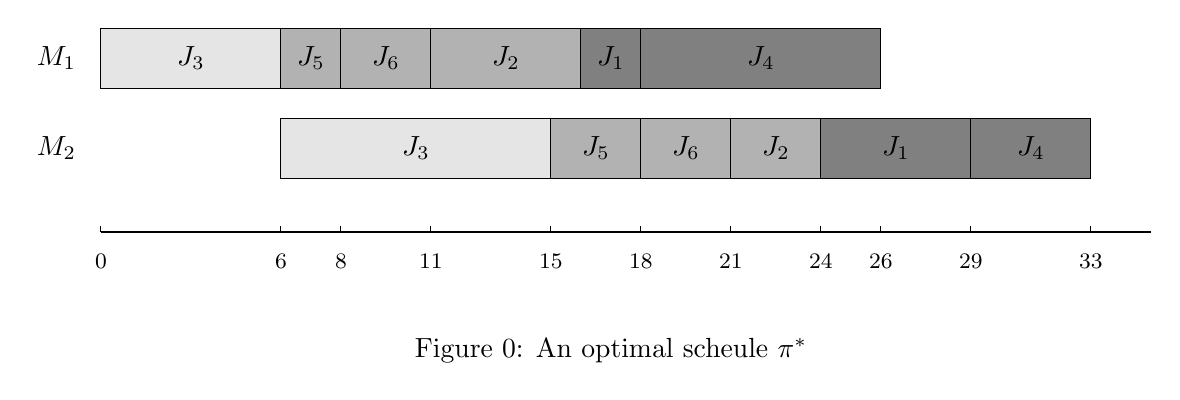
\begin{tikzpicture}[x=0.15in, y=0.3in]
                % machine index
                \node[anchor=east] at (-0.5,5.5) {$M_1$};
                \node[anchor=east] at (-0.5,4) {$M_2$};

                % block 1: weight 5 (J_3)
                \draw[fill=gray!20] (0,5)   rectangle (6,6)   node[midway] {$J_3$};
                % block 2: weight 3 (J_5, J_6, J_2)
                \draw[fill=gray!60] (6,5)   rectangle (8,6)   node[midway] {$J_5$};
                \draw[fill=gray!60] (8,5)   rectangle (11,6)  node[midway] {$J_6$};
                \draw[fill=gray!60] (11,5)  rectangle (16,6)  node[midway] {$J_2$};
                % block 3: weight 2 (J_1, J_4)
                \draw[fill=gray!100] (16,5)  rectangle (18,6)  node[midway] {$J_1$};
                \draw[fill=gray!100] (18,5)  rectangle (26,6)  node[midway] {$J_4$};

                % block 1
                \draw[fill=gray!20] (6,3.5)  rectangle (15,4.5)  node[midway] {$J_3$};
                % block 2
                \draw[fill=gray!60] (15,3.5)  rectangle (18,4.5)  node[midway] {$J_5$};
                \draw[fill=gray!60] (18,3.5)  rectangle (21,4.5)  node[midway] {$J_6$};
                \draw[fill=gray!60] (21,3.5)  rectangle (24,4.5)  node[midway] {$J_2$};
                % block 3
                \draw[fill=gray!100] (24,3.5)  rectangle (29,4.5)  node[midway] {$J_1$};
                \draw[fill=gray!100] (29,3.5)  rectangle (33,4.5)  node[midway] {$J_4$};

                % x-axis
                \draw[thick] (0,2.6) -- (35,2.6);
                \foreach \x/\label in {0/0, 6/6, 8/8, 11/11, 15/15, 18/18, 21/21, 24/24, 26/26, 29/29, 33/33} {
                    \draw (\x,2.6) -- (\x,2.7);
                    \node[below, font=\footnotesize] at (\x,2.4) {\label};
                }

                % caption
                \node[below] at (17,1) {Figure~\thefigure: An optimal scheule $\pi^*$};  \label{fig:exam-3};
            \end{tikzpicture}
        \end{figure}

        \subsection{An FPTAS for fixed number of weights} \label{sec:fptas}

        Let $0 < \epsilon \leq 1$ be real, and let $\delta=1+\epsilon/(2n)$.
        Define the function $\Delta(\cdot)$ on $[0, +\infty)$ by
        \begin{equation} \label{eq-function}
            \Delta(z)=\lfloor \log_{\delta} z \rfloor ~~ (z \geq 1), ~~~~~ \Delta(0)=-1.
        \end{equation}
        Equivalently, if $k$ is an integer that satisfies $\delta^k \leq z < \delta^{k+1}$, then $\Delta(z)=k$.

        For fixed $K$, we apply the geometric rounding technique to transform \Cref{alg:dp} into an FPTAS (which we call \Cref{alg-FPTAS}).
        In contrast to \Cref{alg:dp}, the proposed algorithm may remove some non-dominated states in the tuple set generation procedure.
        Let $\mathcal{H}_j^{\epsilon}$ be the set of tuples generated by \Cref{alg-FPTAS} in the $j$-th iteration.
        For each tuple $(X_1, X_2, \ldots, X_K) \in \mathcal{H}_j^{\epsilon}$, define its label to be $(Y_1, Y_2, \ldots, Y_K)$, where $X_k=(A_k, B_k, C_k, L_k)$ for $k=1, 2, \ldots, K$; the first $K-1$ labels are
        \begin{equation*}
            Y_k=(\Delta(A_k), \Delta(B_k), \Delta(C_k), L_k), ~~ 1 \leq k \leq K-1,
        \end{equation*}
        while the last label is
        \begin{equation*}
            Y_K=(\Delta(A_K), \Delta(B_K), L_K).
        \end{equation*}
        By construction, for each $1 \leq k \leq K$ with $A_k \geq 1$, the rounded value $\delta^{\Delta(A_k)}$ approximates $A_k$ up to a small multiplicative error; likewise, $\delta^{\Delta(B_k)}$ and $\delta^{\Delta(C_k)}$ approximate $B_k$ and $C_k$, respectively.
        Hence, whenever two tuples share a label, one of them is eliminated during tuple elimination procedure.
        A formal description of \Cref{alg-FPTAS} is given below.

        \begin{algorithm}[H]
            \small
            \linespread{1.2}\selectfont
            \SetAlgoLined
            \DontPrintSemicolon
            \caption{An FPTAS for $F2 \mid \mid C_{\max}^w$}  \label{alg-FPTAS}
            \KwIn{Job set $\mathcal{J}$; error parameter $\epsilon$; job parameters $a_j$, $b_j$, $w_j$, and $g_j$ for $j=1, 2, \ldots, n$; $K$ distinct weights with $W_1> W_2 > \cdots > W_K$.}
            \BlankLine
            \textbf{Step 1.} [Preprocessing] Renumber jobs in $\mathcal{J}$ according to Johnson' rule (\Cref{alg:Johnson}). \;

            \textbf{Step 2.} [Initialization] Set $\delta=1+\epsilon/(2n)$. Let  $S_0=\Big(\underbrace{(0,0,0,0),\ldots,(0,0,0,0)}_{K\text{ copies}}\Big)$, and let $R_0=\Big(\underbrace{(-1, -1, -1, 0),\ldots,(-1, -1, -1, 0)}_{K-1\text{ copies}}, (-1, -1, 0)\Big)$ be its label. Initialize $\mathcal{H}_0^{\epsilon}=\{S_0\}$ and $\mathcal{H}_j^{\epsilon}=\emptyset$ for $j=1, 2, \ldots, n$. \;

            \textbf{Step 3.} [Generation of sets $\mathcal{H}_1^{\epsilon}, \mathcal{H}_2^{\epsilon}, \ldots, \mathcal{H}_n^{\epsilon}$]

            \For{$j=1$ \KwTo $n$}
            {
                \For{each $(X_1, X_2, \ldots, X_K) \in \mathcal{H}_{j-1}^{\epsilon}$ with $X_k=(A_k, B_k, C_k, L_k)$, $k=1, 2, \ldots, K$}
                {
                    \For{$k=1$ \KwTo $g_j$}
                    {
                        $A'_k = A_k+a_j$, $B'_k = B_k+b_j$, $C'_k = \max\{C_{k-1}, A_{k-1}+a_j\}+b_j$, $L'_k= w_j$. \;

                        $X'_k=(A'_k, B'_k, C'_k, L'_k)$. \;

                        \eIf{$k \leq K-1$}
                        {
                            $Y'_k=(\Delta(A'_k), \Delta(B'_k), \Delta(C'_k), L'_k)$. \;
                        }
                        {
                            $Y'_K=(\Delta(A'_K), \Delta(B'_K), L'_K)$. \;
                        }

                        Add the tuple $(X_1, \ldots, X_{k-1}, X'_k, X_{k+1}, \ldots, X_K)$ to $\mathcal{H}_j^{\epsilon}$ and attach the associated label $(Y_1, \ldots, Y_{k-1}, Y'_k, Y_{k+1}, \ldots, Y_K)$ to it. \;
                    }
                }
                [Elimination] Among tuples in $\mathcal{H}_j^{\epsilon}$ sharing identical labels, retain only the one with the smallest $C_K$. \;
            }

            \textbf{Step 4.} [Computation of objective values for the tuples in $\mathcal{H}_n^{\epsilon}$]

            \For{each $X=(X_1, X_2, \ldots, X_K) \in \mathcal{H}_n^{\epsilon}$ with $X_k=(A_k, B_k, C_k, L_k)$, $k=1, 2, \ldots, K$}
            {
                Perform the same operations as in Step 4 of \Cref{alg:dp}.
            }

            \textbf{Step 5.} [Result] Compute $C_{\max}^w(X')=\min \{C_{\max}^w(X): X \in \mathcal{H}_n^{\epsilon}\}$ and recover the corresponding approximate schedule $\pi'$ from $X'$ by backtracking. \;

            \KwOut{The approximate schedule $\pi'$.}
        \end{algorithm}

        In \Cref{alg-FPTAS}, the box-elimination operation considers coordinate values that increase geometrically.
        Multiplicative errors can occur if, during tuple elimination, each label is represented by the smallest $C_X$ coordinates inside its box rather than by its exact value.
        Nevertheless, the lemma below demonstrates that the tuples left after elimination form a good approximation to those produced by \Cref{alg:dp}.

        \begin{lemma}\label{lem:approx}
        Given any tuple $(X_1, X_2, \ldots, X_K) \in \mathcal{H}_j$ generated by \Cref{alg:dp}, where $X_k=(A_k, B_k, C_k, L_k)$ for $k=1, 2, \ldots, K$, \Cref{alg-FPTAS} returns a tuple $(\widetilde{X_1}, \widetilde{X_2}, \ldots, \widetilde{X_K}) \in \mathcal{H}_j^{\epsilon}$, with $\widetilde{X_k}=(\widetilde{A_k}, \widetilde{B_k}, \widetilde{C_k}, L_k)$, such that
            \begin{equation} \label{Eq-conditions}
                \widetilde{A_k} \leq \delta^j A_k, ~~ \widetilde{B_k} \leq \delta^j B_k, ~~ \widetilde{C_k} \leq \delta^j C_k, ~~ k=1, 2, \ldots, K.
            \end{equation}
        \end{lemma}

        \begin{proof}
        We prove the result by induction on $j=1, 2, \ldots, n$.
        For the base case $j=1$, $J_1$ can be assigned to each of the $g_1$ schedules (each induced by a block) in \Cref{alg:dp} and \Cref{alg-FPTAS}.
        Since these $g_1$ tuples receive distinct labels in \Cref{alg-FPTAS}, it follows that $\mathcal{H}_1^{\epsilon}=\mathcal{H}_1$, so \cref{Eq-conditions} holds for $j=1$.

        Assume that \cref{Eq-conditions} holds for $j-1$ (the induction hypothesis), where $j \geq 2$.
        Let $(X_1, X_2, \ldots, X_K) \in \mathcal{H}_j$ be a tuple obtained from \Cref{alg:dp} for the first $j$ jobs, where $X_k=(A_k, B_k, C_k, L_k)$ for $k=1, 2, \ldots, K$.
        When implementing \Cref{alg:dp}, the tuple $(X_1, X_2, \ldots, X_K)$ is constructed from a tuple $(X'_1, X'_2, \ldots, X'_K) \in \mathcal{H}_{j-1}$, where $X'_k=(A'_k, B'_k, C'_k, L'_k)$ for $k=1, 2, \ldots, K$.
        Specifically, $J_j$ is assigned to one of the $g_j$ schedules corresponding to $(X'_1, X'_2, \ldots, X'_K)$ for the first $j-1$ jobs.
        Based on the induction hypothesis, there exists a tuple $(\widetilde{X'_1}, \widetilde{X'_2}, \ldots, \widetilde{X'_K}) \in \mathcal{H}_{j-1}^{\epsilon}$, where $\widetilde{X'_k}=(\widetilde{A'_k}, \widetilde{B'_k}, \widetilde{C'_k}, L'_k)$, such that
            \begin{equation} \label{Eq-prev}
                \widetilde{A'_k}  \leq \delta^{j-1} A'_k, ~~ \widetilde{B'_k} \leq \delta^{j-1} B'_k, ~~ \widetilde{C'_k} \leq \delta^{j-1} C'_k, ~~ k=1, 2, \ldots, K.
            \end{equation}
        To prove that \cref{Eq-conditions} holds for $j$, consider the $g_j$ possible cases in which $J_j$ is assigned to one of these schedules.

        Let $J_j$ be assigned to the $h$-th schedule in \Cref{alg:dp} for some $h \in \{1, 2, \ldots, g_j\}$.
        Then
            \begin{equation} \label{Eq-rec-1}
                \begin{aligned}
                    A_k & =A'_k, ~~ B_k=B'_k ~~, C_k=C'_k ~~, L_k=L'_k, ~~ k \in \{1, 2, \ldots, K\} \setminus \{h\}; \\
                    A_h & =A'_h+a_j, ~~ B_h=B'_h+b_j, ~~ C_h=\max \{C'_h, A'_h+a_j\}+b_j, ~~ L_h=w_j.
                \end{aligned}
            \end{equation}
        Since $(\widetilde{X'_1}, \widetilde{X'_2}, \ldots, \widetilde{X'_K}) \in \mathcal{H}_{j-1}^{\epsilon}$, the tuple $(\widetilde{X'_1}, \widetilde{X'_2}, \ldots, \widetilde{X'_{h-1}}, \overline{X'_h}, \widetilde{X'_{h+1}}, \ldots, \widetilde{X'_K})$ is added to $\mathcal{H}_j^{\epsilon}$ in \Cref{alg-FPTAS}, where $\overline{X'_h}=(\overline{A'_h}, \overline{B'_h}, \overline{C'_h}, \overline{L'_h})$ is defined by
            \begin{equation} \label{Eq-rec-2}
                \overline{A'_h}=\widetilde{A'_h}+a_j, ~~ \overline{B'_h}=\widetilde{B'_h}+b_j, ~~ \overline{C'_h}=\max \{\widetilde{C'_h}, \widetilde{A'_h}+a_j\}+b_j, ~~ \overline{L'_h}=w_j.
            \end{equation}
        Because two tuples can share a label, $(\widetilde{X'_1}, \widetilde{X'_2}, \ldots, \widetilde{X'_{h-1}}, \overline{X'_h}, \widetilde{X'_{h+1}}, \ldots, \widetilde{X'_K})$ may be discarded in \Cref{alg-FPTAS} in favor of another tuple $(\widetilde{X_1}, \widetilde{X_2}, \ldots, \widetilde{X_K}) \in \mathcal{H}_j^{\epsilon}$, where $\widetilde{X_k}=(\widetilde{A_k}, \widetilde{B_k}, \widetilde{C_k}, \widetilde{L_k})$ for $k=1, 2, \ldots, K$.
        For this tuple, by \eqref{Eq-prev}--\eqref{Eq-rec-2} and the construction in \Cref{alg-FPTAS}, we have
            \begin{equation} \label{Eq-fin-1}
                \left \{
                \begin{aligned}
                    \widetilde{A_k} &\leq \delta \widetilde{A'_k} \leq \delta^j A'_k = \delta^j A_k \\
                    \widetilde{B_k} &\leq \delta \widetilde{B'_k} \leq \delta^j B'_k = \delta^j B_k \\
                    \widetilde{L_k} &= \overline{L'_k} = L'_k = L_k
                \end{aligned}
                \right. \qquad \qquad \text{if} ~~ k \in \{1, 2, \ldots, K\}\setminus\{h\};
            \end{equation}
            \begin{equation} \label{Eq-fin-2}
                \left \{
                \begin{aligned}
                    \widetilde{A_h} &\leq \delta \overline{A'_h} = \delta(\widetilde{A'_h}+a_j) \leq \delta(\delta^{j-1}A'_h+a_j)
                    \leq \delta^j(A'_h+a_j) = \delta^j A_h \\
                    \widetilde{B_h} &\leq \delta \overline{B'_h} = \delta(\widetilde{B'_h}+b_j) \leq \delta(\delta^{j-1}B'_h+b_j)
                    \leq \delta^j(B'_h+b_j) = \delta^j B_h \\
                    \widetilde{L_h} &= \overline{L'_h}=w_j=L_h
                \end{aligned}
                \right. ;
            \end{equation}
            \begin{equation} \label{Eq-fin-3}
                \left \{
                \begin{aligned}
                    \widetilde{C_k} & \leq \delta \widetilde{C'_k} \leq \delta^j C'_k = \delta^j C_k && \text{if} ~~ k \in \{1, 2, \ldots, K-1\}\setminus \{h\}\\
                    \widetilde{C_K} & \leq \widetilde{C'_K} \leq \delta^{j-1} C'_K \leq \delta^j C_K  &&  \text{if} ~~ K \neq h
                \end{aligned}
                \right. ;
            \end{equation}
            \begin{equation} \label{Eq-fin-4}
                \left \{
                \begin{aligned}
                    \widetilde{C_h} & \leq \delta \overline{C'_h} = \delta (\max \{\widetilde{C'_h}, \widetilde{A'_h}+a_j\}+b_j) \\
                    & \leq \delta (\max \{\delta^{j-1}C'_h, \delta^{j-1}A'_h+a_j\}+b_j) && \text{if}~~ h \neq K\\
                    & \leq \delta^j (\max\{C'_h, A'_h+a_j\}+b_j) = \delta^j C_h \\
                    \widetilde{C_K} & \leq \overline{C'_K} = \max \{\widetilde{C'_K} \widetilde{A'_K}+a_j\}+b_j \\
                    & \leq  \max \{\delta^{j-1}C'_K, \delta^{j-1}A'_K+a_j\}+b_j && \text{if} ~~ h = K    \\
                    & \leq \delta^{j-1} (\max\{C'_K, A'_K+a_j\}+b_j) \leq \delta^j C_K
                \end{aligned}
                \right. .
            \end{equation}

        By \cref{Eq-fin-1}-\cref{Eq-fin-4}, \cref{Eq-conditions} holds for $j$ when $J_j$ is assigned to the $h$-th schedule.
        Since $h$ is arbitrary, this covers every possible assignment of $J_j$.
        Thus, the induction step is established for $j$.
        \end{proof}

        To analyze the approximation error and time complexity of \Cref{alg-FPTAS}, we use the following two well-known inequalities.
        The first follows because $f(x)=x \ln x-(x-1)$ is increasing on $[1, +\infty)$ and $f(1)=0$.
        The second follows because $g(x)=(1+\frac{x}{n})^n-(1+2x)$ is convex on $[0, 1]$, with $g(0)=0$ and $g(1) \leq 0$.

        \begin{lemma} \label{Lem-ineq-1}
        For any real $x \geq 1$, $\ln x \geq (x-1)/x$.
        \end{lemma}

        \begin{lemma} \label{Lem-ineq-2}
        For any real $0 < x \leq 1$, $(1+x/n)^n \leq 1+2x$.
        \end{lemma}

        \begin{theorem} \label{Thm-FPTAS}
        For fixed $K$, \Cref{alg-FPTAS} is an FPTAS for $F2 \mid \mid C_{\max}^w$ with $O((n^{3K}/\epsilon^{3K-1}) (\log P)^{3K-1})$ running time.
        \end{theorem}

        \begin{proof}
        We first bound the approximation error of the algorithm.
        Let $\pi'$ be the approximate schedule returned by \cref{alg-FPTAS}, and let $\pi_{\mathrm{opt}}$ be the optimal schedule returned by \Cref{alg:dp}.
        Denote by $(X_1^*, X_2^*, \ldots, X_K^*) \in \mathcal{H}_n$ the tuple corresponding to $\pi_{\mathrm{opt}}$, where $X_k^*=(A_k^*, B_k^*, C_k^*, L_k^*)$ for $k=1, 2, \ldots, K$.
        By \cref{eq-4.2:block-makespan} and \cref{eq-4.2:block-weighted makespan}, we have
            \begin{equation} \label{Lem-4.3-fptas-1}
                C_{\max}^w(\pi_{\mathrm{opt}}) =\max_{1 \leq k \leq K} \Big\{W_k \max_{0 \leq h \leq k-1} \Big(\sum_{i=1}^h A_i^* +C_{h+1}^* + \sum_{i=h+2}^k B_i^* \Big)\Big\}.
            \end{equation}

        By \Cref{lem:approx}, there exists a tuple $(\widetilde{X_1^*}, \widetilde{X_2^*}, \ldots, \widetilde{X_K^*}) \in \mathcal{H}_n^{\epsilon}$ generated by \Cref{alg-FPTAS}, with $\widetilde{X_k^*}=(\widetilde{A_k^*}, \widetilde{B_k^*}, \widetilde{C_k^*}, L_k^*)$, such that
            \begin{equation} \label{Lem-4.3-fptas-2}
                \widetilde{A_k^*} \leq \delta^n A_k^*, ~~ \widetilde{B_k^*} \leq \delta^n B_k^*, ~~ \widetilde{C_k^*} \leq \delta^n C_k^*, ~~  k=1, 2, \ldots, K.
            \end{equation}
        Let $\widetilde{\pi_{\mathrm{opt}}}$ be the schedule corresponding to $(\widetilde{X_1^*}, \widetilde{X_2^*}, \ldots, \widetilde{X_K^*})$.
        Again by \cref{eq-4.2:block-makespan} and \cref{eq-4.2:block-weighted makespan}, we have
            \begin{equation} \label{Lem-4.3-fptas-3}
                C_{\max}^w(\widetilde{\pi_{\mathrm{opt}}}) =\max_{1 \leq k \leq K} \Big\{W_k \max_{0 \leq h \leq k-1} \Big(\sum_{i=1}^h \widetilde{A_i^*} +\widetilde{C_{h+1}^*} + \sum_{i=h+2}^k \widetilde{B_i^*} \Big)\Big\}.
            \end{equation}
        Recall that $0 < \epsilon \leq 1$ and $\delta=1+\epsilon/(2n)$.
        Then by \Cref{Lem-ineq-2} and \cref{Lem-4.3-fptas-1}--\cref{Lem-4.3-fptas-3}, we have
            \begin{equation*}
                \begin{aligned}
                    C_{\max}^w(\widetilde{\pi_{\mathrm{opt}}}) & \leq \max_{1 \leq k \leq K} \Big\{W_k \max_{0 \leq h \leq k-1} \Big(\sum_{i=1}^h \delta^n A_i^* +\delta^n C_{h+1}^* + \sum_{i=h+2}^k \delta^n B_i^* \Big)\Big\} \\
                    & = \delta^n \max_{1 \leq k \leq K} \Big\{W_k \max_{0 \leq h \leq k-1} \Big(\sum_{i=1}^h  A_i^* + C_{h+1}^* + \sum_{i=h+2}^k B_i^* \Big)\Big\} \\
                    & \leq (1+\epsilon)C_{\max}^w(\pi_{\mathrm{opt}}).
                \end{aligned}
            \end{equation*}
        Thus, from the execution of \Cref{alg-FPTAS}, it returns an approximate schedule $\pi'$ with $C_{\max}^w(\pi') \leq C_{\max}^w(\widetilde{\pi_{\mathrm{opt}}}) \leq (1+\epsilon)C_{\max}^w(\pi_{\mathrm{opt}})$.

        We next bound the time complexity of the algorithm.
        Step 1 sorts in $O(n\log n)$ time, and Step 2 initializes in $O(n)$ time.
        In Step 3, at most one tuple is retained per label after elimination.
        For each $(X_1, X_2, \ldots, X_K) \in \mathcal{H}_j^{\epsilon}$ ($j=1, 2, \ldots, n$), the corresponding label is  $(Y_1, Y_2, \ldots, Y_K)$, where $X_k=(A_k, B_k, C_k, L_k)$ for $k=1, 2, \ldots, K$, $Y_k=(\Delta(A_k), \Delta(B_k), \Delta(C_k), L_k)$ for $1 \leq k \leq K-1$, and $Y_K=(\Delta(A_K), \Delta(B_K), L_K)$.
        Note that $A_k \leq P$, $B_k \leq P$, $C_k \leq 2P$, and $L_k \in \{0, W_k, W_{k+1}, \ldots, W_K\}$ for $k=1, 2, \ldots, K$.
        By \Cref{Lem-ineq-1}, the number of distinct values attained by $\Delta(A_k)$ is upper bounded by $1+\lfloor \log_{\delta} P \rfloor = 1+ \lfloor \ln P / \ln \delta \rfloor \leq 1+ \lfloor (1+2n/ \epsilon) \ln P \rfloor =O((n/ \epsilon) \log P)$.
        Analogously, the number of distinct values attained by $\Delta(B_k)$ and $\Delta(C_k)$ are also upper bounded by $O((n/\epsilon) \log P)$.
        Because each tuple yields at most $K$ new tuples, after elimination, the number of retained tuples in $\mathcal{H}_j^{\epsilon}$ is upper bounded by $O((n^{3K-1}/\epsilon^{3K-1}) (\log P)^{3K-1})$.
        Summing the cost of Step 3 over its $n$ iterations gives $O((n^{3K}/\epsilon^{3K-1}) \log P)$ time.
        Step 4 computes the objective value of each tuple in $\mathcal{H}_n^{\epsilon}$ in $O(K)$ time, and thus requires $O((n^{3K-1}/\epsilon^{3K-1}) (\log P)^{3K-1})$ time in total.
        Step 5 has the same time complexity.
        Consequently, the algorithm runs in $O((n^{3K}/\epsilon^{3K-1}) (\log P)^{3K-1})$ time.
        \end{proof}

        \subsection{The bounded max-to-min weight ratio} \label{sec:bounded_weight}

        Consider the bounded max-to-min ratio weight case where $w_{\max}/w_{\min} \leq C$ for some constant $C$.
        Here, $w_{\max}=\max_{1 \leq j \leq n} \{w_j\}$ is the maximum weight of the $n$ jobs, and $w_{\min}=\min_{1 \leq j \leq n} \{w_j\}$ is the minimum weight.
        The proof of \Cref{thm:nphard} demonstrates that the problem remains $\mathcal{NP}$-hard even when $C=2$.

        Let $0 < \epsilon \leq 1$ be a real number.
        For $j=1, 2, \ldots, n$, we round each weight $w_j$ down to the nearest value of the form  $w_{\min}(1+\epsilon/2)^k$, i.e., $\overline{w_j}=w_{\min}(1+\epsilon/2)^{\theta_j}$, where $\theta_j$ is the unique integer satisfying
        \begin{equation} \label{eq-4.4-PTAS-1}
            w_{\min}(1+\epsilon/2)^{\theta_j} \leq w_j < w_{\min}(1+\epsilon/2)^{\theta_j+1}.
        \end{equation}


        By combining job-weight rounding with the FPTAS in \Cref{sec:fptas}, a PTAS for the bounded max-to-min ratio weight case is given as follows.

        \begin{algorithm}[H]
            \small
            \linespread{1.2}\selectfont
            \SetAlgoLined
            \DontPrintSemicolon
            \caption{A PTAS for $F2 \mid \mid C_{\max}^w$ with bounded max-to-min weight ratio}  \label{Alg-PTAS}
            \KwIn{Job set $\mathcal{J}$; error parameter $\epsilon$; job parameters $a_j$, $b_j$, and $w_j$ for $j=1, 2, \ldots, n$.}
            \BlankLine
            \textbf{Step 1.} Construct the rounded instance $\mathcal{I}'$ from the original instance $\mathcal{I}$: replace each job $J_j$ by $J'_j$ with $w'_j=w_{\min}(1+\epsilon/2)^{\theta_j}$, where $\theta_j$ is the integer given by \cref{eq-4.4-PTAS-1}; keep all other job parameters unchanged. \;

            \textbf{Step 2.} Let $W_1 >W_2> \cdots >W_K$ be the ordered sequence of distinct rounded weights in $\mathcal{I}'$. Run \Cref{alg-FPTAS} on $\mathcal{I}'$ to obtain a $(1+\epsilon/3)$-approximation schedule $\pi_{\epsilon}$. \;

            \KwOut{The approximate schedule $\pi_{\epsilon}$.}
        \end{algorithm}

        For a schedule $\pi$, let $C_{\max}^w(\pi, \mathcal{I})=\max_{1 \leq j \leq n}\{ w_{\pi(j)} C_{\pi(j)}(\pi,\mathcal{I})\}$ and $C_{\max}^w(\pi,\mathcal{I}')=\max_{1 \leq j \leq n}\{ w'_{\pi(j)} C_{\pi(j)}(\pi, \mathcal{I}')\}$ denote its weighted makespan on instances $\mathcal{I}$ and $\overline{\mathcal{I}}$, respectively.
        Here, $C_{\pi(j)}(\pi,\mathcal{I})$ and $C_{\pi(j)}(\pi, \mathcal{I}')$ are the completion times of $J_{\pi(j)}$ under $\pi$ on $\mathcal{I}$ and $\mathcal{I}'$, respectively.

        \begin{theorem} \label{Theorem-PTAS}
        When $w_{\max}/w_{\min} \leq C$, \Cref{Alg-PTAS} is a PTAS for $F2 \mid \mid C_{\max}^w$ with $O((n^{O(1/\epsilon)}/\epsilon^{O(1/\epsilon)}) (\log P)^{O(1/\epsilon)})$ running time.
        \end{theorem}

        \begin{proof}
        Let $\pi_{\mathrm{opt}}$ be an optimal schedule for $\mathcal{I}$, and let $\pi'_{\mathrm{opt}}$ be an optimal schedule for $\mathcal{I}'$.
        Because $\mathcal{I}$ and $\mathcal{I}'$ differ only in their job weights, a fixed schedule $\pi$ yields the same job completion times on both instances, i.e., $C_{\pi(j)}(\pi,\mathcal{I})=C_{\pi(j)}(\pi, \mathcal{I}')$.
        Thus, from the fact that $w'_j \leq w_j < (1+\epsilon/2) w'_j$, $j=1, 2, \ldots, n$, we have
            \begin{equation} \label{Eq-4.4-PTAS-1}
                C_{\max}^w(\pi_{\epsilon}, \mathcal{I}) < (1+\epsilon/2)C_{\max}^w(\pi_{\epsilon}, \mathcal{I}')
            \end{equation}
        and
            \begin{equation} \label{Eq-4.4-PTAS-2}
                C_{\max}^w(\pi'_{\mathrm{opt}}, \mathcal{I}') \leq C_{\max}^w(\pi_{\mathrm{opt}}, \mathcal{I}') \leq C_{\max}^w(\pi_{\mathrm{opt}}, \mathcal{I}).
            \end{equation}
        Since $\pi_{\epsilon}$ is a $(1+\epsilon/3)$-approximation schedule for $\mathcal{I}'$, we have
            \begin{equation} \label{Eq-4.4-PTAS-3}
                C_{\max}^w(\pi_{\epsilon}, \mathcal{I}') \leq (1+\epsilon/3) C_{\max}^w(\pi'_{\mathrm{opt}}, \mathcal{I}').
            \end{equation}
        Then, \cref{Eq-4.4-PTAS-1}--\cref{Eq-4.4-PTAS-3} imply that
            \begin{equation*}
                C_{\max}^w(\pi_{\epsilon}, \mathcal{I}) \leq (1+\epsilon/2) (1+\epsilon/3) C_{\max}^w(\pi'_{\mathrm{opt}}, \mathcal{I}')  \leq  (1+\epsilon)C_{\max}^w(\pi_{\mathrm{opt}},\mathcal{I}).
            \end{equation*}

        Let $\mathcal{W}=\{\overline{w_j}: 1 \leq j \leq n\}$ be the set of distinct rounded job weights in $\mathcal{I}'$, and let $K=|\mathcal{W}|$.
        Since $w_{\max}/w_{\min} \leq C$ and $C$ is a constant, we have $K \leq 1+ \lfloor \log_{1+\epsilon/2} C \rfloor =O(1/\epsilon)$.
        The running time is dominated by Step 2.
        By \Cref{Thm-FPTAS}, it requires $O((n^{3K}/\epsilon^{3K-1}) (\log P)^{3K-1})=O((n^{O(1/\epsilon)}/\epsilon^{O(1/\epsilon)}) (\log P)^{O(1/\epsilon)})$ time.
        Consequently, the overall running time is $O((n^{O(1/\epsilon)}/\epsilon^{O(1/\epsilon)}) (\log P)^{O(1/\epsilon)})$.
        \end{proof}



        \section{Heuristic algorithms} \label{sec:heuristics}
        
        This section presents two heuristic methods for instances that are too large to be solved efficiently 
        by the exact methods: an adaptation of the NEH heuristic, which constructs a schedule through sequential job insertion, 
        and a genetic algorithm, which searches the space of job permutations.
        
        
        \subsection{The LW algorithm} \label{sec:lw}
        
        \cite{Sun2024JOCO} proved that the LW-based greedy algorithm is a $(2-1/m)$-approximation for $Pm \mid \mid C_{\max}^w$. For $F2 \mid \mid C_{\max}^w$, we describe the analogous LW-based algorithm and show that its worst-case approximation ratio is $2$.
        
        \begin{algorithm}[H]
            \small
            \linespread{1.2}\selectfont
            \SetAlgoLined
            \DontPrintSemicolon
            \caption{LW's rule for $F2 \mid \mid C_{\max}^w$} \label{Alg-LW}
            \KwIn{Job set $\mathcal{J}$; job parameters $a_j$, $b_j$, and $w_j$ for $j=1, 2, \ldots, n$.}
            \BlankLine
            \textbf{Step 1.} Renumber the jobs in nonincreasing order of their weights (i.e., the LW order), so that $w_1 \geq w_2 \geq \cdots \geq w_n$. \;
            
            \textbf{Step 2.} Process the jobs in this order on $M_1$ and then on $M_2$, yielding the permutation schedule $\pi_{\mathrm{lw}}$. \;
            
            \KwOut{The resulting schedule $\pi_{\mathrm{lw}}$.}
        \end{algorithm}
        
        \begin{theorem}\label{Thm-LW}
            For $F2 \mid \mid C_{\max}^w$, \Cref{Alg-LW} has a worst-case approximation ratio of $2$, which is tight, and runs in $O(n\log n)$ time.
        \end{theorem}
        
        \begin{proof}
            Since $1 \mid \mid C_{\max}^w$ can be solved in $O(n\log n)$ time by the LW rule \citep{NongChengNg2011EJOR}, we have
            \begin{equation}\label{Eq-LB}
                C_{\max}^w(\pi_{\mathrm{opt}}) \geq LB=\max \Big \{\max_{1 \leq j \leq n} \Big\{w_j \sum_{i=1}^j a_i \Big\}, \max_{1 \leq j \leq n} \Big\{w_j \sum_{i=1}^j b_i\Big\}, \max_{1 \leq j \leq n} \Big\{w_j (a_j+b_j)\Big\} \Big\},
            \end{equation}
            where the first two terms are machine-based lower bounds and the last is a job-based lower bound.   
            
            By construction, \Cref{Alg-LW} yields $\pi_{\mathrm{lw}}(j)=j$ for $j=1, 2, \ldots, n$. Combining \cref{eq:completion} with  \cref{eq:wcmax}, the weighted makespan of $\pi_{lw}$ can be written as 
            \begin{equation}\label{Eq-LW-WC-1}
                C_{\max}^w(\pi_{\mathrm{lw}}) =\max_{1 \leq j \leq n}\Big\{ w_{\pi_{\mathrm{lw}}(j)} C_{\pi_{\mathrm{lw}}(j)}\Big\}=\max_{1 \leq j \leq n} \Big\{w_j \max_{1 \leq i \leq j} \Big (\sum_{h=1}^{i}a_h + \sum_{h=i}^{j}b_h \Big) \Big\}.
            \end{equation}
            
            By \cref{Eq-LB} and \cref{Eq-LW-WC-1}, we have 
            \begin{equation}\label{Eq-LW-WC-2}
                \begin{aligned}
                    C_{\max}^w(\pi_{\mathrm{lw}}) & \leq \max_{1 \leq j \leq n} \Big\{w_j \sum_{h=1}^{j}a_h + w_j \sum_{h=1}^{j}b_h \Big\} \\
                    & \leq \max_{1 \leq j \leq n} \Big\{w_j \sum_{h=1}^{j}a_h \Big\}+\max_{1 \leq j \leq n} \Big\{w_j \sum_{h=1}^{j}b_h \Big\} \\
                    & \leq 2 C_{\max}^w(\pi_{\mathrm{opt}}).
                \end{aligned}
            \end{equation}
            
            To show that the bound is tight, consider an instance with two jobs: $J_1$ has  $a_1=1+\epsilon$, $b_1=\epsilon$, and $w_1= 1+\epsilon$, and $J_2$ has $a_2=\epsilon$, $b_2=1+\epsilon$, and $w_2= 1$, where $\epsilon > 0$ is arbitrarily small. \Cref{Alg-LW} yields the schedule $\pi_{\mathrm{lw}}=(1,2)$ with $C_{\max}^w(\pi_{\mathrm{lw}})=2+\epsilon$, while the optimal schedule is $\pi_{\mathrm{opt}}=(2,1)$ with $C_{\max}^w(\pi_{\mathrm{opt}})=(1+\epsilon)(1+2\epsilon)$. Hence, $C_{\max}^w(\pi_{\mathrm{lw}})/C_{\max}^w(\pi_{\mathrm{opt}}) \to 2$ as $\epsilon \to 0$.
        \end{proof}
        
        \subsection{The NEH algorithm} \label{sec:neh}
        
        The NEH heuristic is a classical insertion-based constructive method for the permutation flow-shop scheduling problem. In the formulation of Nawaz et al. \cite{NawazEnscoreHam1983Omega}, jobs are placed sequentially: at each iteration, an unassigned job is examined at every feasible position in the current partial schedule, and the position with the smallest resulting makespan is retained. This procedure has proven competitive in diverse scheduling settings. In addition, NEH has recently been used in scheduling research as a construction to be refined \citep{PukaSkalnaIwona2024COR}, as a rule for assigning jobs in distributed lot-streaming and cascaded flow shops \citep{ShaoShaoPi2023ESWA,WangPanSang2024RCIM}, and as the core of composite heuristics for a constrained distributed group scheduling problem \citep{WangPanGao2024CIE}. For the $C_{\max}^w$ objective, two properties are relevant. First, jobs with large total processing time $a_j+b_j$ tend to lengthen the schedule and should be scheduled early to avoid delaying other jobs. Second, for a fixed makespan, jobs with larger weight $w_j$ benefit more from earlier positions, since this reduces the objective value. Accordingly, we prioritize jobs by nonincreasing $a_j+b_j$, breaking ties by nonincreasing $w_j$, and insert each job into the position yielding the smallest objective value. The detailed procedure is presented in \Cref{Alg-NEH}. At iteration $k$, evaluating all $k$ insertion positions requires $O(k^2)$ time, so the overall running time is $O(n^3)$.
        
        \begin{algorithm}[H]
            \small
            \linespread{1.2}\selectfont
            \SetAlgoLined
            \DontPrintSemicolon
            \caption{NEH heuristic for $F2 \mid \mid C_{\max}^w$}\label{Alg-NEH}
            \KwIn{Job set $\mathcal{J}$; job parameters $a_j$, $b_j$, and $w_j$ for $j=1, 2, \ldots, n$.}
            \BlankLine
            \textbf{Step 1.} [Preprocessing] Renumber the jobs in $\mathcal{J}$ by nonincreasing $a_j+b_j$, and the ties are broken by nonincreasing $w_j$.  \;
            
            \textbf{Step 2.} [Initialization] $\pi \gets (J_{1})$. \;
            
            \textbf{Step 3.} [Insertion] \For{$k=2$ \KwTo $n$}
            {
                $\pi \gets$ insert $J_{k}$ into $\pi$ at a position that minimizes $C_{\max}^w$. \;
            }
            \KwOut{The resulting schedule $\pi$.}
        \end{algorithm}
        
        \subsection{The genetic algorithm} \label{sec:ga}
        
        Genetic algorithms (GAs) are commonly applied in scheduling, where operators are tailored to problem structure. Recent flow-shop studies have developed genetic operators for blocking constraints \citep{deAthaydePrataFuchigami2024JIM},  sequence-independent setup times and non-interruption requirements \citep{QiaoWuHeLi2022ESA}, and energy consumption under variable machine speeds \citep{WangWang2023EAAI}. For the $C_{\max}^w$ objective, an optimal schedule consists of weight-based blocks, and jobs within each block follow Johnson's order (\Cref{lem:block-johnson}). Using this structural property, we design a weight-block genetic algorithm (which we call \Cref{Alg-GA}) with a weight-class-based mutation operator as its core component.
        
        Each chromosome encodes a job permutation. The initial population contains the schedule constructed from Johnson's rule  and $N-1$ adjacent-swap variants, where $N$ is the population size. Johnson's rule ignores job weights, but it provides a structured, makespan-minimizing schedule as a starting point for the weight-aware search. Parents are selected by fitness-based binary tournament. Partially mapped crossover is applied with probability $p_c$ and mutation with probability $p_m$. Elitist selection keeps the $N$ best individuals from the combined parent and offspring pools, preserving the best solution across generations.
        
        The distinctive component of \Cref{Alg-GA} is its weight-class mutation operator. Rather than moving individual jobs, it removes a whole weight class, keeps the relative order of its jobs, and reinserts the class as a block at the position yielding the smallest $C_{\max}^w$. The class is chosen with equal probability either from classes containing a job that attains the current $C_{\max}^w$ or uniformly at random. Repositioning all jobs of a class at once makes use of the block structure. A forward move can delay the jobs passed over, so the move is not guaranteed to improve the schedule; its retention is left to the subsequent selection. To improve schedule quality, a local search sequentially relocates the $k$ jobs with the largest $w_j C_j$ values to the position minimizing $C_{\max}^w$. It stops when a round produces no improvement in $C_{\max}^w$ or after $G$ rounds. 

        \begin{algorithm}[H]
            \small
            \linespread{1.2}\selectfont
            \SetAlgoLined
            \DontPrintSemicolon
            \caption{The weight-block genetic algorithm (WBGA) for $F2 \mid \mid C_{\max}^w$} \label{Alg-GA}
            
            \KwIn{Job set $\mathcal{J}$; population size $N$; generations $G$; offspring
                $\lambda$; probabilities $p_c$, $p_m$; reinsertion count $k$.}
            \BlankLine
            \textbf{Step 1.} [Initialization] Build $P_0$ from Johnson's rule and $N-1$ adjacent-swap variants; evaluate all individuals. \;
            
            \textbf{Step 2.} [Evolution] \For{$g=1$ \KwTo $G$}
            {
                \textbf{Selection} Form the mating pool $M_g$ from $P_{g-1}$ by binary tournament selection. \;
                 
                \textbf{Crossover} \While{$|O_g|<\lambda$}
                {
                    Draw two parents from $M_g$. With probability $p_c$, apply crossover to obtain two children; otherwise copy the parents. Add the children to $O_g$ one by one, stoping once $|O_g|=\lambda$. \;
                }
                
                \textbf{Mutation} For each child, apply block mutation with probability $p_m$; evaluate all children using \cref{eq:completion} and \cref{eq:wcmax}. \;
                
                \textbf{Survival} $P_g \gets$ the $N$ schedules with the minimum $C_{\max}^w$ in $P_{g-1}\cup O_g$. \;
            }
            
            $\pi^{*} \gets$ the schedule with the minimum $C_{\max}^w$ in $P_G$. \;
            
            \textbf{Step 3.} [Local search] \Repeat{no reinsertion lowers $C_{\max}^w(\pi^{*})$, or $G$ rounds have been performed.}
            {
                Let $J_{1}, J_{2}, \ldots, J_{k}$ be the jobs of $\pi^{*}$ with the largest $w_jC_j$ value. \;
                
                For each $J_i$ and each position $r$, construct the schedule obtained by removing $J_i$ and reinserting it into position $r$, and evaluate it using \cref{eq:completion} and \cref{eq:wcmax}. Let $\pi'$ denote the best resulting schedule. \;
                
                \If{$C_{\max}^w(\pi')<C_{\max}^w(\pi^{*})$}
                {
                  $\pi^{*} \gets \pi'$ \;
                }
            }
            \KwOut{The best schedule $\pi^{*}$.}
        \end{algorithm}


        \section{Numerical experiments} \label{sec:experiments}


        All algorithms were implemented in Python 3.13 and run on a computer equipped with an Intel Core Ultra 5 230F processor and 16 GB of RAM, running Windows 11.
        The $\mathbf{MILP}$ model was solved using Gurobi 13.0 with a single thread.
        Each method was run once per instance, with a time limit of 600 s.
        All objective values were evaluated using the same recurrence \cref{eq:completion}.

        \subsection{Experimental setup} \label{sec:setup}

        An instance consists of $n$ jobs, where each job $J_j$ has processing times $a_j$ and $b_j$ on machines $M_1$ and $M_2$, respectively, and a weight $w_j$.
        The processing times are independently drawn from $\mathcal{U}(1,40)$ or $\mathcal{U}(1,80)$, while the weights are drawn from $\{1,\ldots,K\}$.
        A fixed random seed is assigned to each configuration to ensure that all methods are tested on identical instances and that the experiments are reproducible.

        Three groups of test instances are considered, covering both processing-time ranges.
        Each configuration contains 20 independently generated instances.
        Group 1 evaluates the performance of $\mathbf{DP}$ across different instance sizes, with $n\in\{40,60,80,100\}$, $K=2$, and weights restricted to $\{1,10\}$, resulting in eight configurations.
        Group 2 compares the $\mathbf{MILP}$ model with $\mathbf{LW}$, $\mathbf{NEH}$, and $\mathbf{GA}$ for $n=10,15,\ldots,60$, resulting in 22 configurations.
        Group 3 compares the three heuristic methods, $\mathbf{LW}$, $\mathbf{NEH}$, and $\mathbf{GA}$, on larger instances with $n=100,120,\ldots,400$, resulting in 32 configurations.
        Groups 2 and 3 use $K=30$, with weights drawn from $\{1,2,\ldots,30\}$.

        For $\mathbf{GA}$, the population size is set to $N=\min\{20,\max\{6,\lceil n/2\rceil\}\}$.
        The number of generations is set to $G=\max\{2,\lfloor n/4\rfloor\}$ for small instances and $G=11+\lfloor(n-100)/10\rfloor$ for large instances.
        These parameter settings are designed to balance solution quality and computational time.

        Algorithmic performance is evaluated using the relative percentage gap:
        \begin{equation}\label{eq:gap}
            \text{gap}_A =
            \frac{z_A-z_{\text{base}}}{z_{\text{base}}}\times 100\%,
        \end{equation}
        where $z_A$ is the objective value obtained by $\mathbf{method\ A}$ $( \mathbf{DP}, \mathbf{LW}, \mathbf{NEH}, \mathbf{GA})$, and $z_{\text{base}}$ is the reference value.
        For the small-scale instances, $z_{\text{base}}$ is the $\mathbf{MILP}$ optimum whenever optimality is proven by the solver.
        For the large-scale instances, it is the lower bound $LB$ of \cref{Eq-LB}, the maximum of the two machine-based bounds and the job-based bound.
        Thus, large-scale gaps measure the distance from a common lower bound rather than from competing heuristic solutions.
        This bound is tight only when the heaviest jobs also appear earliest.

        \subsection{Computational results} \label{sec:results}

        The five methods exhibit different trade-offs between solution quality, computational cost and generality, with none dominating across all instances.


        \subsubsection{The dynamic program} \label{sec:results_dp}

        The $\mathbf{DP}$ is the only exact method considered and guarantees optimality whenever it terminates.
        It solves all twenty instances in seven of the eight configurations, with mean running times of 1.47 s and 4.98 s for forty-job instances under $[1,40]$ and $[1,80]$, respectively (\Cref{tab:results-dp-k2}).
        However, its running time increases rapidly with instance size.
        Under $[1,40]$, the mean running time rises from 1.47 s for forty jobs to 89.59 s for one hundred jobs, a 61-fold increase, while the mean objective value increases by only a factor of 2.5.
        Expanding the processing-time range to $[1,80]$ further increases the mean running time by factors of 2.9--3.7.
        For one hundred-job instances under $[1,80]$, six of the twenty instances reach the 600 s time limit, and the remaining fourteen require an average of 329.01 s.
        Moreover, the $\mathbf{DP}$ cannot handle a third weight class due to memory limitations, restricting its applicability to $K=2$.
        These results indicate that the $\mathbf{DP}$ is effective for relatively small instances with few distinct weights but has limited scalability.

        \begin{table}[H]
            \resultstable
            \caption{The dynamic program, $K=2$}
            \label{tab:results-dp-k2}
            \setlength{\tabcolsep}{9.0pt}
            \begin{tabular*}{\resultstabwidth}{@{}l r r r r r @{\hspace{14pt}} r r r r r@{}}
                \toprule
                \multirow{3}{*}{$n$} & \multicolumn{5}{c}{$a_j,b_j\in[1,40]$} & \multicolumn{5}{c}{$a_j,b_j\in[1,80]$} \\
                \cmidrule(lr){2-6}\cmidrule(lr){7-11}
                & \multicolumn{2}{c}{$W C_{\max}$} & \multicolumn{2}{c}{time (ms)} & opt. & \multicolumn{2}{c}{$W C_{\max}$} & \multicolumn{2}{c}{time (ms)} & opt. \\
                \cmidrule(lr){2-3}\cmidrule(lr){4-5}\cmidrule(lr){7-8}\cmidrule(lr){9-10}
                & avg & max & avg & max &  & avg & max & avg & max &  \\
                \midrule
                $40$ & $4335.0$ & $5480.0$ & $1.5\mathrm{e}3$ & $4.3\mathrm{e}3$ & $20/20$ & $8604.5$ & $10590.0$ & $5.0\mathrm{e}3$ & $2.4\mathrm{e}4$ & $20/20$ \\
                $60$ & $6340.0$ & $7270.0$ & $1.4\mathrm{e}4$ & $3.1\mathrm{e}4$ & $20/20$ & $12344.5$ & $15020.0$ & $5.3\mathrm{e}4$ & $1.1\mathrm{e}5$ & $20/20$ \\
                $80$ & $8221.0$ & $9750.0$ & $4.5\mathrm{e}4$ & $1.1\mathrm{e}5$ & $20/20$ & $17341.5$ & $19580.0$ & $1.3\mathrm{e}5$ & $2.8\mathrm{e}5$ & $20/20$ \\
                $100$ & $10647.0$ & $12350.0$ & $9.0\mathrm{e}4$ & $1.7\mathrm{e}5$ & $20/20$ & $21544.3$ & $24240.0$ & $3.3\mathrm{e}5$ & $6.0\mathrm{e}5$ & $14/20$ \\
                \bottomrule
            \end{tabular*}
            \par\vspace{2pt}
            {\scriptsize Averages at $n=100$ on $[1,80]$ cover the $14$ instances settled within the
                $600$\,s limit; the other six are cut short.}
        \end{table}

        \subsubsection{The small scale} \label{sec:results_small}

        \Crefrange{tab:results-small-40}{tab:results-small-80} report the objective values, running times and gaps of the four methods under $[1,40]$ and $[1,80]$, respectively.

        The $\mathbf{MILP}$ model solves 436 of the 440 instances to optimality, providing reference values.
        Under $[1,40]$, its mean running time increases from 70 ms for ten jobs to 160.7 s for sixty jobs, with four instances at the largest size reaching the time limit.
        The wider processing-time range roughly doubles the objective values but has no consistent effect on running time.

        $\mathbf{NEH}$ outperforms $\mathbf{LW}$ in all 22 configurations, achieving overall mean gaps of 3.14\% and 5.77\%, respectively, and worst individual-instance gaps of 24.89\% and 21.49\%.
        This improvement comes at a higher computational cost: $\mathbf{NEH}$ takes 2.66 ms on average, compared with 0.02 ms for $\mathbf{LW}$, reflecting its sequential evaluation of insertion positions versus the latter's single-pass construction.
        Thus, $\mathbf{LW}$ is preferable when computational efficiency outweighs solution quality.

        The $\mathbf{GA}$ shows the opposite trend, with its mean gap decreasing from 12.61\% to 1.70\% under $[1,40]$ and from 14.29\% to 3.90\% under $[1,80]$ as the number of jobs increases from ten to sixty.
        It outperforms both constructive methods at sixty jobs.
        Nevertheless, its overall mean gap remains the largest (10.07\%), and its performance is non-monotonic, with a worst individual-instance gap of 57.53\% at twenty-five jobs.
        This may reflect the limited search budget at smaller sizes, where six individuals and two generations for ten jobs provide insufficient opportunities to establish the block structure.
        Its mean running time rises from 0.64 ms to 1.69 s, remaining well below that of the $\mathbf{MILP}$ model.
        At sixty jobs, however, the mean gaps of the three heuristics differ by less than three percentage points.

        Overall, the small-scale results distinguish the methods primarily by computational cost.
        The $\mathbf{MILP}$ model alone certifies optimality but becomes increasingly expensive as the instance size grows.
        Among the heuristics, $\mathbf{NEH}$ offers the best quality-cost trade-off, $\mathbf{LW}$ sacrifices some solution quality for substantially lower running times, while $\mathbf{GA}$ performs worst in solution quality and incurs the highest computational cost (\Cref{fig:gap-small}).
        Hence, $\mathbf{NEH}$ is the preferred heuristic for small instances unless optimality certification is required.
        The effectiveness of the additional search effort invested in $\mathbf{GA}$ on larger instances is examined next.

        \begin{table}[H]
            \resultstable
            \caption{The small scale, $a_j,b_j\in[1,40]$: MILP, LW, NEH, GA}
            \label{tab:results-small-40}
            \setlength{\tabcolsep}{3.95pt}
            \scriptsize
            \begin{tabular*}{\resultstabwidth}{@{}l r r r r @{\hspace{5pt}} r r r r @{\hspace{5pt}} r r r r @{\hspace{5pt}} r r r r@{}}
                \toprule
                \multirow{3}{*}{$n$} & \multicolumn{4}{c}{MILP} & \multicolumn{4}{c}{LW} & \multicolumn{4}{c}{NEH} & \multicolumn{4}{c}{GA} \\
                \cmidrule(lr){2-5}\cmidrule(lr){6-9}\cmidrule(lr){10-13}\cmidrule(lr){14-17}
                & \multicolumn{2}{c}{$W C_{\max}$} & \multicolumn{2}{c}{time (ms)} & \multicolumn{2}{c}{gap} & \multicolumn{2}{c}{time (ms)} & \multicolumn{2}{c}{gap} & \multicolumn{2}{c}{time (ms)} & \multicolumn{2}{c}{gap} & \multicolumn{2}{c}{time (ms)} \\
                \cmidrule(lr){2-3}\cmidrule(lr){4-5}\cmidrule(lr){6-7}\cmidrule(lr){8-9}\cmidrule(lr){10-11}\cmidrule(lr){12-13}\cmidrule(lr){14-15}\cmidrule(lr){16-17}
                & avg & max & avg & max & avg & max & avg & max & avg & max & avg & max & avg & max & avg & max \\
                \midrule
                $10$ & $2607.8$ & $4369.0$ & $7.0\mathrm{e}1$ & $1.2\mathrm{e}2$ & $7.3$ & $17.2$ & $8.8\mathrm{e}{-3}$ & $2.5\mathrm{e}{-2}$ & $\mathbf{3.4}$ & $24.9$ & $7.3\mathrm{e}{-2}$ & $7.9\mathrm{e}{-2}$ & $12.6$ & $30.6$ & $6.4\mathrm{e}{-1}$ & $7.2\mathrm{e}{-1}$ \\
                $15$ & $3758.2$ & $5049.0$ & $1.9\mathrm{e}2$ & $4.7\mathrm{e}2$ & $6.8$ & $16.9$ & $9.9\mathrm{e}{-3}$ & $1.9\mathrm{e}{-2}$ & $\mathbf{2.1}$ & $8.5$ & $1.9\mathrm{e}{-1}$ & $2.0\mathrm{e}{-1}$ & $18.2$ & $49.5$ & $2.6\mathrm{e}0$ & $2.9\mathrm{e}0$ \\
                $20$ & $4811.3$ & $5967.0$ & $5.6\mathrm{e}2$ & $1.9\mathrm{e}3$ & $6.2$ & $19.9$ & $1.3\mathrm{e}{-2}$ & $2.3\mathrm{e}{-2}$ & $\mathbf{2.7}$ & $11.7$ & $3.8\mathrm{e}{-1}$ & $4.1\mathrm{e}{-1}$ & $12.1$ & $33.0$ & $1.0\mathrm{e}1$ & $1.1\mathrm{e}1$ \\
                $25$ & $5590.8$ & $7059.0$ & $1.5\mathrm{e}3$ & $5.7\mathrm{e}3$ & $5.6$ & $21.5$ & $1.4\mathrm{e}{-2}$ & $2.5\mathrm{e}{-2}$ & $\mathbf{3.7}$ & $17.5$ & $7.0\mathrm{e}{-1}$ & $7.4\mathrm{e}{-1}$ & $15.3$ & $57.5$ & $2.8\mathrm{e}1$ & $3.3\mathrm{e}1$ \\
                $30$ & $6888.1$ & $8025.0$ & $2.8\mathrm{e}3$ & $1.0\mathrm{e}4$ & $5.6$ & $14.9$ & $1.4\mathrm{e}{-2}$ & $2.6\mathrm{e}{-2}$ & $\mathbf{3.9}$ & $10.8$ & $1.1\mathrm{e}0$ & $1.2\mathrm{e}0$ & $11.6$ & $26.7$ & $6.2\mathrm{e}1$ & $7.0\mathrm{e}1$ \\
                $35$ & $7719.7$ & $9373.0$ & $8.4\mathrm{e}3$ & $3.6\mathrm{e}4$ & $5.7$ & $12.2$ & $1.4\mathrm{e}{-2}$ & $2.4\mathrm{e}{-2}$ & $\mathbf{3.2}$ & $13.8$ & $1.8\mathrm{e}0$ & $1.8\mathrm{e}0$ & $12.8$ & $38.7$ & $1.2\mathrm{e}2$ & $1.3\mathrm{e}2$ \\
                $40$ & $8830.8$ & $10309.0$ & $2.1\mathrm{e}4$ & $1.2\mathrm{e}5$ & $4.9$ & $10.6$ & $1.7\mathrm{e}{-2}$ & $3.0\mathrm{e}{-2}$ & $\mathbf{2.4}$ & $6.2$ & $2.5\mathrm{e}0$ & $2.6\mathrm{e}0$ & $7.0$ & $17.5$ & $2.4\mathrm{e}2$ & $2.5\mathrm{e}2$ \\
                $45$ & $9669.2$ & $11791.0$ & $3.1\mathrm{e}4$ & $2.5\mathrm{e}5$ & $6.0$ & $19.0$ & $1.8\mathrm{e}{-2}$ & $3.8\mathrm{e}{-2}$ & $\mathbf{3.7}$ & $10.3$ & $3.5\mathrm{e}0$ & $3.7\mathrm{e}0$ & $8.8$ & $24.7$ & $4.1\mathrm{e}2$ & $4.5\mathrm{e}2$ \\
                $50$ & $10904.9$ & $12558.0$ & $8.4\mathrm{e}4$ & $5.1\mathrm{e}5$ & $4.5$ & $13.0$ & $1.8\mathrm{e}{-2}$ & $3.1\mathrm{e}{-2}$ & $\mathbf{3.6}$ & $8.4$ & $4.8\mathrm{e}0$ & $4.9\mathrm{e}0$ & $6.5$ & $22.9$ & $6.7\mathrm{e}2$ & $7.3\mathrm{e}2$ \\
                $55$ & $11858.3$ & $14340.0$ & $1.1\mathrm{e}5$ & $5.2\mathrm{e}5$ & $4.7$ & $10.9$ & $2.7\mathrm{e}{-2}$ & $4.7\mathrm{e}{-2}$ & $\mathbf{3.1}$ & $11.9$ & $6.2\mathrm{e}0$ & $6.4\mathrm{e}0$ & $4.2$ & $14.6$ & $1.0\mathrm{e}3$ & $1.2\mathrm{e}3$ \\
                $60$ & $13051.7$ & $15330.0$ & $1.6\mathrm{e}5$ & $6.0\mathrm{e}5$ & $4.7$ & $11.7$ & $2.5\mathrm{e}{-2}$ & $4.2\mathrm{e}{-2}$ & $4.3$ & $8.8$ & $8.0\mathrm{e}0$ & $8.2\mathrm{e}0$ & $\mathbf{1.7}$ & $8.2$ & $1.7\mathrm{e}3$ & $1.9\mathrm{e}3$ \\
                \bottomrule
            \end{tabular*}
        \end{table}

        \begin{table}[H]
            \resultstable
            \caption{The small scale, $a_j,b_j\in[1,80]$: MILP, LW, NEH, GA}
            \label{tab:results-small-80}
            \setlength{\tabcolsep}{3.95pt}
            \scriptsize
            \begin{tabular*}{\resultstabwidth}{@{}l r r r r @{\hspace{5pt}} r r r r @{\hspace{5pt}} r r r r @{\hspace{5pt}} r r r r@{}}
                \toprule
                \multirow{3}{*}{$n$} & \multicolumn{4}{c}{MILP} & \multicolumn{4}{c}{LW} & \multicolumn{4}{c}{NEH} & \multicolumn{4}{c}{GA} \\
                \cmidrule(lr){2-5}\cmidrule(lr){6-9}\cmidrule(lr){10-13}\cmidrule(lr){14-17}
                & \multicolumn{2}{c}{$W C_{\max}$} & \multicolumn{2}{c}{time (ms)} & \multicolumn{2}{c}{gap} & \multicolumn{2}{c}{time (ms)} & \multicolumn{2}{c}{gap} & \multicolumn{2}{c}{time (ms)} & \multicolumn{2}{c}{gap} & \multicolumn{2}{c}{time (ms)} \\
                \cmidrule(lr){2-3}\cmidrule(lr){4-5}\cmidrule(lr){6-7}\cmidrule(lr){8-9}\cmidrule(lr){10-11}\cmidrule(lr){12-13}\cmidrule(lr){14-15}\cmidrule(lr){16-17}
                & avg & max & avg & max & avg & max & avg & max & avg & max & avg & max & avg & max & avg & max \\
                \midrule
                $10$ & $5029.9$ & $7345.0$ & $5.1\mathrm{e}1$ & $1.0\mathrm{e}2$ & $8.1$ & $17.5$ & $8.5\mathrm{e}{-3}$ & $1.8\mathrm{e}{-2}$ & $\mathbf{0.8}$ & $5.7$ & $7.2\mathrm{e}{-2}$ & $7.8\mathrm{e}{-2}$ & $14.3$ & $47.5$ & $6.1\mathrm{e}{-1}$ & $6.8\mathrm{e}{-1}$ \\
                $15$ & $7182.1$ & $8624.0$ & $2.9\mathrm{e}2$ & $1.8\mathrm{e}3$ & $7.7$ & $19.7$ & $9.5\mathrm{e}{-3}$ & $2.0\mathrm{e}{-2}$ & $\mathbf{2.4}$ & $14.5$ & $1.9\mathrm{e}{-1}$ & $2.1\mathrm{e}{-1}$ & $15.9$ & $37.5$ & $2.6\mathrm{e}0$ & $2.9\mathrm{e}0$ \\
                $20$ & $9328.9$ & $12103.0$ & $4.5\mathrm{e}2$ & $1.8\mathrm{e}3$ & $4.5$ & $11.8$ & $1.2\mathrm{e}{-2}$ & $2.9\mathrm{e}{-2}$ & $\mathbf{2.6}$ & $9.6$ & $3.8\mathrm{e}{-1}$ & $4.1\mathrm{e}{-1}$ & $16.3$ & $39.1$ & $1.0\mathrm{e}1$ & $1.2\mathrm{e}1$ \\
                $25$ & $10816.3$ & $14100.0$ & $1.6\mathrm{e}3$ & $4.6\mathrm{e}3$ & $4.7$ & $16.2$ & $1.2\mathrm{e}{-2}$ & $2.1\mathrm{e}{-2}$ & $\mathbf{2.1}$ & $7.9$ & $7.0\mathrm{e}{-1}$ & $7.4\mathrm{e}{-1}$ & $15.7$ & $37.6$ & $2.8\mathrm{e}1$ & $3.0\mathrm{e}1$ \\
                $30$ & $12972.5$ & $16005.0$ & $3.2\mathrm{e}3$ & $9.5\mathrm{e}3$ & $5.6$ & $11.7$ & $1.5\mathrm{e}{-2}$ & $2.9\mathrm{e}{-2}$ & $\mathbf{2.6}$ & $13.6$ & $1.2\mathrm{e}0$ & $1.2\mathrm{e}0$ & $14.4$ & $34.2$ & $6.1\mathrm{e}1$ & $6.6\mathrm{e}1$ \\
                $35$ & $15093.3$ & $17667.0$ & $8.7\mathrm{e}3$ & $4.1\mathrm{e}4$ & $7.0$ & $18.1$ & $1.8\mathrm{e}{-2}$ & $3.1\mathrm{e}{-2}$ & $\mathbf{4.3}$ & $7.9$ & $1.8\mathrm{e}0$ & $1.8\mathrm{e}0$ & $11.5$ & $27.5$ & $1.2\mathrm{e}2$ & $1.3\mathrm{e}2$ \\
                $40$ & $16757.4$ & $20146.0$ & $2.4\mathrm{e}4$ & $1.5\mathrm{e}5$ & $6.3$ & $20.8$ & $1.8\mathrm{e}{-2}$ & $3.1\mathrm{e}{-2}$ & $\mathbf{2.4}$ & $7.6$ & $2.5\mathrm{e}0$ & $2.6\mathrm{e}0$ & $5.5$ & $15.9$ & $2.5\mathrm{e}2$ & $2.7\mathrm{e}2$ \\
                $45$ & $19621.4$ & $24528.0$ & $6.8\mathrm{e}4$ & $3.8\mathrm{e}5$ & $4.8$ & $12.3$ & $1.6\mathrm{e}{-2}$ & $1.9\mathrm{e}{-2}$ & $\mathbf{2.8}$ & $11.9$ & $3.5\mathrm{e}0$ & $3.7\mathrm{e}0$ & $5.3$ & $13.1$ & $4.2\mathrm{e}2$ & $4.5\mathrm{e}2$ \\
                $50$ & $21338.0$ & $25044.0$ & $7.7\mathrm{e}4$ & $4.8\mathrm{e}5$ & $6.2$ & $12.4$ & $1.9\mathrm{e}{-2}$ & $3.0\mathrm{e}{-2}$ & $\mathbf{3.8}$ & $11.1$ & $4.7\mathrm{e}0$ & $4.8\mathrm{e}0$ & $4.2$ & $12.0$ & $6.6\mathrm{e}2$ & $7.4\mathrm{e}2$ \\
                $55$ & $23019.6$ & $25376.0$ & $1.4\mathrm{e}5$ & $4.7\mathrm{e}5$ & $5.0$ & $11.4$ & $2.2\mathrm{e}{-2}$ & $3.9\mathrm{e}{-2}$ & $5.0$ & $16.2$ & $6.2\mathrm{e}0$ & $6.5\mathrm{e}0$ & $\mathbf{3.5}$ & $14.7$ & $1.1\mathrm{e}3$ & $1.2\mathrm{e}3$ \\
                $60$ & $26079.5$ & $31320.0$ & $1.9\mathrm{e}5$ & $6.0\mathrm{e}5$ & $5.0$ & $13.5$ & $2.8\mathrm{e}{-2}$ & $4.4\mathrm{e}{-2}$ & $4.4$ & $15.4$ & $8.0\mathrm{e}0$ & $8.2\mathrm{e}0$ & $\mathbf{3.9}$ & $20.8$ & $1.7\mathrm{e}3$ & $1.8\mathrm{e}3$ \\
                \bottomrule
            \end{tabular*}
        \end{table}

        \begin{figure}[H]
            \centering
            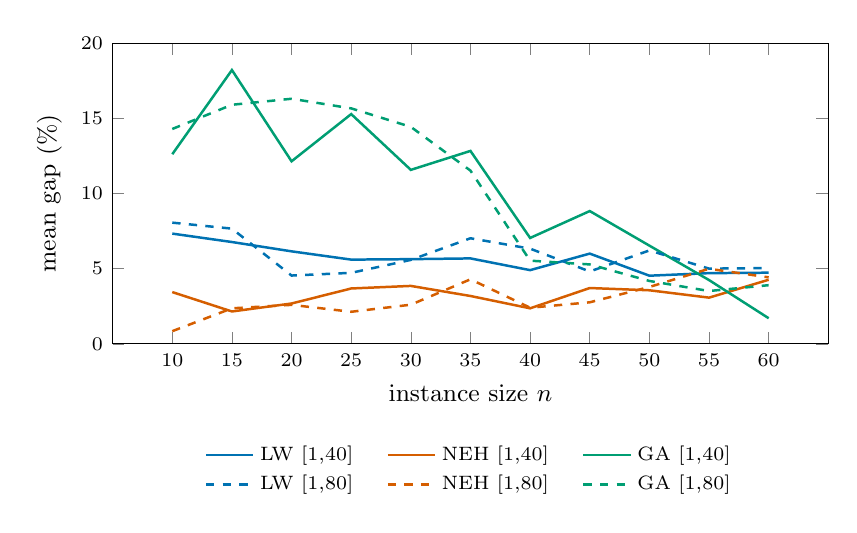
\begin{tikzpicture}
                \begin{axis}[
                    width=0.88\textwidth, height=5.4cm,
                    xlabel={instance size $n$}, ylabel={mean gap (\%)},
                    xtick={10,15,20,25,30,35,40,45,50,55,60}, xticklabels={10,15,20,25,30,35,40,45,50,55,60},
                    ymin=0, ymax=20,
                    tick label style={font=\scriptsize}, label style={font=\small},
                    every axis plot/.append style={line width=0.9pt},
                    legend columns=3,
                    legend style={font=\scriptsize, at={(0.5,-0.30)}, anchor=north, draw=none,
                        /tikz/every even column/.append style={column sep=10pt}},
                    ]
                    \addplot[apxblue] coordinates {(10,7.33) (15,6.77) (20,6.15) (25,5.60) (30,5.63) (35,5.68) (40,4.90) (45,6.00) (50,4.53) (55,4.70) (60,4.73)};
                    \addlegendentry{LW $[1{,}40]$}
                    \addplot[nehred] coordinates {(10,3.44) (15,2.15) (20,2.68) (25,3.68) (30,3.85) (35,3.18) (40,2.36) (45,3.71) (50,3.56) (55,3.07) (60,4.26)};
                    \addlegendentry{NEH $[1{,}40]$}
                    \addplot[gagreen] coordinates {(10,12.61) (15,18.21) (20,12.14) (25,15.28) (30,11.57) (35,12.83) (40,7.04) (45,8.83) (50,6.53) (55,4.24) (60,1.70)};
                    \addlegendentry{GA $[1{,}40]$}
                    \addplot[apxblue, dashed] coordinates {(10,8.06) (15,7.66) (20,4.54) (25,4.72) (30,5.58) (35,7.02) (40,6.33) (45,4.81) (50,6.21) (55,5.00) (60,5.04)};
                    \addlegendentry{LW $[1{,}80]$}
                    \addplot[nehred, dashed] coordinates {(10,0.84) (15,2.36) (20,2.59) (25,2.13) (30,2.60) (35,4.29) (40,2.40) (45,2.76) (50,3.78) (55,4.99) (60,4.42)};
                    \addlegendentry{NEH $[1{,}80]$}
                    \addplot[gagreen, dashed] coordinates {(10,14.29) (15,15.90) (20,16.30) (25,15.66) (30,14.43) (35,11.52) (40,5.53) (45,5.28) (50,4.18) (55,3.51) (60,3.90)};
                    \addlegendentry{GA $[1{,}80]$}
                \end{axis}
            \end{tikzpicture}
            \caption{Mean relative gap of the LW and the two heuristics on the small scale, against the optimum the model returned. A solid line is $a_j,b_j\in[1,40]$, a dashed line $a_j,b_j\in[1,80]$.}
            \label{fig:gap-small}
        \end{figure}


        \subsubsection{The large scale} \label{sec:results_large}

        \Crefrange{tab:results-large-40}{tab:results-large-80} report the gaps and running times of the three heuristics under $[1,40]$ and $[1,80]$, respectively.

        On the large scale, the ranking varies with instance size.
        The $\mathbf{LW}$ achieves the smallest overall mean gap of 2.67\% across the 32 configurations, with a worst individual-instance gap of 12.92\%, followed by $\mathbf{NEH}$ at 5.06\% and 10.77\%, respectively.
        By contrast, the $\mathbf{GA}$ improves substantially with instance size: its mean gap decreases from 18.33\% to 0.62\% under $[1,40]$ and from 16.01\% to 0.82\% under $[1,80]$ between one hundred and four hundred jobs.
        It overtakes $\mathbf{NEH}$ at 220 jobs under both ranges and $\mathbf{LW}$ at 220 and 240 jobs, respectively.

        For sufficiently large instances, the $\mathbf{GA}$ achieves the best solution quality at a higher computational cost.
        It obtains the best objective values in 328 of the 640 instances, compared with 250 for $\mathbf{LW}$ and 62 for $\mathbf{NEH}$, while its mean running time is 42.2 s, compared with 0.74 s and 0.09 ms, respectively.
        Unlike the $\mathbf{DP}$, it also handles instances with 30 distinct weight classes.
        The processing-time range has little effect on the overall ranking: the mean gaps of $\mathbf{LW}$, $\mathbf{NEH}$ and $\mathbf{GA}$ are 2.74\%, 4.75\% and 4.44\% under $[1,40]$, and 2.59\%, 5.36\% and 4.96\% under $[1,80]$, respectively.
        These gaps are measured against the lower bound $LB$ defined in \cref{Eq-LB}, which is tight only when the heaviest jobs appear earliest; they therefore measure deviations from $LB$ rather than true optimality gaps.

        Overall, the large-scale results highlight the trade-off between solution quality and computational time.
        The $\mathbf{LW}$ is the fastest method and achieves the smallest overall mean gap, while $\mathbf{NEH}$ offers intermediate performance at negligible computational cost.
        The $\mathbf{GA}$ achieves the best solutions on sufficiently large instances but requires substantially more time (\Cref{fig:gap-large}).
        The choice therefore depends on whether computational speed or solution quality is the priority.

        \begin{table}[H]
            \resultstable
            \caption{The large scale, $a_j,b_j\in[1,40]$: LW, NEH, GA}
            \label{tab:results-large-40}
            \setlength{\tabcolsep}{8.15pt}
            \begin{tabular*}{\resultstabwidth}{@{}l r r r r @{\hspace{14pt}} r r r r @{\hspace{14pt}} r r r r@{}}
                \toprule
                \multirow{3}{*}{$n$} & \multicolumn{4}{c}{LW} & \multicolumn{4}{c}{NEH} & \multicolumn{4}{c}{GA} \\
                \cmidrule(lr){2-5}\cmidrule(lr){6-9}\cmidrule(lr){10-13}
                & \multicolumn{2}{c}{gap} & \multicolumn{2}{c}{time (ms)} & \multicolumn{2}{c}{gap} & \multicolumn{2}{c}{time (ms)} & \multicolumn{2}{c}{gap} & \multicolumn{2}{c}{time (ms)} \\
                \cmidrule(lr){2-3}\cmidrule(lr){4-5}\cmidrule(lr){6-7}\cmidrule(lr){8-9}\cmidrule(lr){10-11}\cmidrule(lr){12-13}
                & avg & max & avg & max & avg & max & avg & max & avg & max & avg & max \\
                \midrule
                $100$ & $\mathbf{4.4}$ & $10.0$ & $3.4\mathrm{e}{-2}$ & $6.2\mathrm{e}{-2}$ & $5.2$ & $9.7$ & $3.7\mathrm{e}1$ & $6.3\mathrm{e}1$ & $18.3$ & $29.2$ & $9.7\mathrm{e}2$ & $1.1\mathrm{e}3$ \\
                $120$ & $\mathbf{3.5}$ & $6.5$ & $4.8\mathrm{e}{-2}$ & $1.1\mathrm{e}{-1}$ & $4.8$ & $10.0$ & $6.1\mathrm{e}1$ & $6.3\mathrm{e}1$ & $13.8$ & $32.1$ & $1.8\mathrm{e}3$ & $1.8\mathrm{e}3$ \\
                $140$ & $\mathbf{3.0}$ & $6.6$ & $5.8\mathrm{e}{-2}$ & $1.2\mathrm{e}{-1}$ & $5.3$ & $8.5$ & $9.7\mathrm{e}1$ & $1.0\mathrm{e}2$ & $9.3$ & $20.6$ & $3.1\mathrm{e}3$ & $3.2\mathrm{e}3$ \\
                $160$ & $\mathbf{3.4}$ & $7.5$ & $6.7\mathrm{e}{-2}$ & $1.3\mathrm{e}{-1}$ & $4.2$ & $7.4$ & $1.4\mathrm{e}2$ & $1.5\mathrm{e}2$ & $6.5$ & $14.4$ & $5.1\mathrm{e}3$ & $5.3\mathrm{e}3$ \\
                $180$ & $\mathbf{2.6}$ & $7.8$ & $7.1\mathrm{e}{-2}$ & $9.8\mathrm{e}{-2}$ & $4.9$ & $7.6$ & $2.0\mathrm{e}2$ & $2.2\mathrm{e}2$ & $5.3$ & $13.8$ & $8.0\mathrm{e}3$ & $8.4\mathrm{e}3$ \\
                $200$ & $\mathbf{2.6}$ & $5.6$ & $7.5\mathrm{e}{-2}$ & $1.2\mathrm{e}{-1}$ & $4.4$ & $7.6$ & $2.7\mathrm{e}2$ & $2.9\mathrm{e}2$ & $4.5$ & $15.7$ & $1.2\mathrm{e}4$ & $1.3\mathrm{e}4$ \\
                $220$ & $3.4$ & $8.6$ & $8.7\mathrm{e}{-2}$ & $1.1\mathrm{e}{-1}$ & $5.0$ & $8.2$ & $3.6\mathrm{e}2$ & $3.8\mathrm{e}2$ & $\mathbf{3.0}$ & $11.7$ & $1.8\mathrm{e}4$ & $1.8\mathrm{e}4$ \\
                $240$ & $\mathbf{2.8}$ & $5.9$ & $8.5\mathrm{e}{-2}$ & $1.1\mathrm{e}{-1}$ & $4.7$ & $7.3$ & $4.9\mathrm{e}2$ & $5.1\mathrm{e}2$ & $2.8$ & $7.4$ & $2.6\mathrm{e}4$ & $2.7\mathrm{e}4$ \\
                $260$ & $2.6$ & $6.0$ & $1.0\mathrm{e}{-1}$ & $1.5\mathrm{e}{-1}$ & $5.4$ & $8.7$ & $5.7\mathrm{e}2$ & $5.8\mathrm{e}2$ & $\mathbf{1.6}$ & $4.7$ & $3.2\mathrm{e}4$ & $3.3\mathrm{e}4$ \\
                $280$ & $2.5$ & $7.8$ & $9.7\mathrm{e}{-2}$ & $1.2\mathrm{e}{-1}$ & $5.1$ & $7.7$ & $7.2\mathrm{e}2$ & $7.4\mathrm{e}2$ & $\mathbf{0.8}$ & $3.9$ & $4.3\mathrm{e}4$ & $4.4\mathrm{e}4$ \\
                $300$ & $2.0$ & $4.9$ & $1.1\mathrm{e}{-1}$ & $1.8\mathrm{e}{-1}$ & $4.9$ & $8.6$ & $9.0\mathrm{e}2$ & $9.1\mathrm{e}2$ & $\mathbf{0.9}$ & $5.0$ & $5.3\mathrm{e}4$ & $5.4\mathrm{e}4$ \\
                $320$ & $3.0$ & $7.6$ & $1.1\mathrm{e}{-1}$ & $1.2\mathrm{e}{-1}$ & $4.4$ & $7.4$ & $1.1\mathrm{e}3$ & $1.1\mathrm{e}3$ & $\mathbf{1.2}$ & $6.3$ & $6.5\mathrm{e}4$ & $6.6\mathrm{e}4$ \\
                $340$ & $1.5$ & $3.7$ & $1.3\mathrm{e}{-1}$ & $2.4\mathrm{e}{-1}$ & $4.7$ & $7.1$ & $1.3\mathrm{e}3$ & $1.3\mathrm{e}3$ & $\mathbf{1.2}$ & $8.0$ & $7.8\mathrm{e}4$ & $7.9\mathrm{e}4$ \\
                $360$ & $2.2$ & $5.5$ & $1.3\mathrm{e}{-1}$ & $1.6\mathrm{e}{-1}$ & $4.7$ & $7.0$ & $1.6\mathrm{e}3$ & $1.6\mathrm{e}3$ & $\mathbf{0.9}$ & $7.1$ & $9.3\mathrm{e}4$ & $9.6\mathrm{e}4$ \\
                $380$ & $2.3$ & $6.2$ & $1.4\mathrm{e}{-1}$ & $1.5\mathrm{e}{-1}$ & $4.5$ & $8.7$ & $1.9\mathrm{e}3$ & $1.9\mathrm{e}3$ & $\mathbf{0.3}$ & $1.5$ & $1.1\mathrm{e}5$ & $1.1\mathrm{e}5$ \\
                $400$ & $2.0$ & $5.9$ & $1.5\mathrm{e}{-1}$ & $1.7\mathrm{e}{-1}$ & $3.9$ & $8.0$ & $2.2\mathrm{e}3$ & $2.2\mathrm{e}3$ & $\mathbf{0.6}$ & $2.7$ & $1.3\mathrm{e}5$ & $1.3\mathrm{e}5$ \\
                \bottomrule
            \end{tabular*}
        \end{table}

        \begin{table}[H]
            \resultstable
            \caption{The large scale, $a_j,b_j\in[1,80]$: LW, NEH, GA}
            \label{tab:results-large-80}
            \setlength{\tabcolsep}{8.15pt}
            \begin{tabular*}{\resultstabwidth}{@{}l r r r r @{\hspace{14pt}} r r r r @{\hspace{14pt}} r r r r@{}}
                \toprule
                \multirow{3}{*}{$n$} & \multicolumn{4}{c}{LW} & \multicolumn{4}{c}{NEH} & \multicolumn{4}{c}{GA} \\
                \cmidrule(lr){2-5}\cmidrule(lr){6-9}\cmidrule(lr){10-13}
                & \multicolumn{2}{c}{gap} & \multicolumn{2}{c}{time (ms)} & \multicolumn{2}{c}{gap} & \multicolumn{2}{c}{time (ms)} & \multicolumn{2}{c}{gap} & \multicolumn{2}{c}{time (ms)} \\
                \cmidrule(lr){2-3}\cmidrule(lr){4-5}\cmidrule(lr){6-7}\cmidrule(lr){8-9}\cmidrule(lr){10-11}\cmidrule(lr){12-13}
                & avg & max & avg & max & avg & max & avg & max & avg & max & avg & max \\
                \midrule
                $100$ & $\mathbf{3.6}$ & $8.9$ & $4.1\mathrm{e}{-2}$ & $1.3\mathrm{e}{-1}$ & $4.6$ & $10.8$ & $3.6\mathrm{e}1$ & $4.1\mathrm{e}1$ & $16.0$ & $30.1$ & $9.6\mathrm{e}2$ & $1.0\mathrm{e}3$ \\
                $120$ & $\mathbf{4.4}$ & $12.9$ & $4.3\mathrm{e}{-2}$ & $7.1\mathrm{e}{-2}$ & $5.4$ & $9.3$ & $6.1\mathrm{e}1$ & $6.2\mathrm{e}1$ & $17.1$ & $38.5$ & $1.8\mathrm{e}3$ & $1.8\mathrm{e}3$ \\
                $140$ & $\mathbf{3.5}$ & $10.7$ & $5.2\mathrm{e}{-2}$ & $9.4\mathrm{e}{-2}$ & $4.4$ & $7.7$ & $9.6\mathrm{e}1$ & $9.9\mathrm{e}1$ & $12.6$ & $25.3$ & $3.1\mathrm{e}3$ & $3.2\mathrm{e}3$ \\
                $160$ & $\mathbf{3.2}$ & $11.4$ & $6.8\mathrm{e}{-2}$ & $1.1\mathrm{e}{-1}$ & $5.8$ & $9.9$ & $1.4\mathrm{e}2$ & $1.5\mathrm{e}2$ & $8.1$ & $25.8$ & $5.1\mathrm{e}3$ & $5.2\mathrm{e}3$ \\
                $180$ & $\mathbf{3.0}$ & $7.3$ & $6.7\mathrm{e}{-2}$ & $9.6\mathrm{e}{-2}$ & $5.3$ & $9.0$ & $2.1\mathrm{e}2$ & $2.5\mathrm{e}2$ & $5.9$ & $14.3$ & $8.3\mathrm{e}3$ & $8.5\mathrm{e}3$ \\
                $200$ & $\mathbf{2.7}$ & $8.6$ & $9.3\mathrm{e}{-2}$ & $2.5\mathrm{e}{-1}$ & $4.7$ & $7.2$ & $2.8\mathrm{e}2$ & $2.9\mathrm{e}2$ & $4.9$ & $10.1$ & $1.2\mathrm{e}4$ & $1.3\mathrm{e}4$ \\
                $220$ & $\mathbf{2.9}$ & $8.0$ & $8.0\mathrm{e}{-2}$ & $1.1\mathrm{e}{-1}$ & $4.8$ & $8.7$ & $3.8\mathrm{e}2$ & $4.0\mathrm{e}2$ & $3.6$ & $9.0$ & $1.8\mathrm{e}4$ & $1.9\mathrm{e}4$ \\
                $240$ & $2.9$ & $6.4$ & $8.9\mathrm{e}{-2}$ & $1.2\mathrm{e}{-1}$ & $6.0$ & $8.9$ & $4.5\mathrm{e}2$ & $4.8\mathrm{e}2$ & $\mathbf{1.9}$ & $6.5$ & $2.4\mathrm{e}4$ & $2.5\mathrm{e}4$ \\
                $260$ & $1.8$ & $5.3$ & $9.1\mathrm{e}{-2}$ & $1.1\mathrm{e}{-1}$ & $5.2$ & $9.3$ & $5.7\mathrm{e}2$ & $5.8\mathrm{e}2$ & $\mathbf{1.6}$ & $8.0$ & $3.2\mathrm{e}4$ & $3.3\mathrm{e}4$ \\
                $280$ & $2.3$ & $4.8$ & $1.0\mathrm{e}{-1}$ & $1.3\mathrm{e}{-1}$ & $5.5$ & $9.2$ & $7.2\mathrm{e}2$ & $7.3\mathrm{e}2$ & $\mathbf{0.8}$ & $4.3$ & $4.3\mathrm{e}4$ & $4.4\mathrm{e}4$ \\
                $300$ & $2.8$ & $6.3$ & $1.0\mathrm{e}{-1}$ & $1.2\mathrm{e}{-1}$ & $5.4$ & $7.5$ & $9.0\mathrm{e}2$ & $9.1\mathrm{e}2$ & $\mathbf{2.0}$ & $11.8$ & $5.3\mathrm{e}4$ & $5.4\mathrm{e}4$ \\
                $320$ & $1.9$ & $4.7$ & $1.2\mathrm{e}{-1}$ & $2.3\mathrm{e}{-1}$ & $5.7$ & $8.5$ & $1.1\mathrm{e}3$ & $1.1\mathrm{e}3$ & $\mathbf{1.4}$ & $6.1$ & $6.5\mathrm{e}4$ & $6.6\mathrm{e}4$ \\
                $340$ & $1.4$ & $3.0$ & $1.2\mathrm{e}{-1}$ & $1.3\mathrm{e}{-1}$ & $5.6$ & $8.6$ & $1.3\mathrm{e}3$ & $1.4\mathrm{e}3$ & $\mathbf{0.8}$ & $3.3$ & $7.8\mathrm{e}4$ & $8.0\mathrm{e}4$ \\
                $360$ & $1.7$ & $3.2$ & $1.3\mathrm{e}{-1}$ & $1.5\mathrm{e}{-1}$ & $5.8$ & $8.2$ & $1.6\mathrm{e}3$ & $1.6\mathrm{e}3$ & $\mathbf{1.1}$ & $7.3$ & $9.3\mathrm{e}4$ & $9.4\mathrm{e}4$ \\
                $380$ & $1.8$ & $4.0$ & $1.4\mathrm{e}{-1}$ & $1.6\mathrm{e}{-1}$ & $5.9$ & $9.1$ & $1.9\mathrm{e}3$ & $1.9\mathrm{e}3$ & $\mathbf{0.8}$ & $2.9$ & $1.1\mathrm{e}5$ & $1.1\mathrm{e}5$ \\
                $400$ & $1.7$ & $4.6$ & $1.5\mathrm{e}{-1}$ & $2.1\mathrm{e}{-1}$ & $5.8$ & $9.1$ & $2.2\mathrm{e}3$ & $2.3\mathrm{e}3$ & $\mathbf{0.8}$ & $2.9$ & $1.3\mathrm{e}5$ & $1.3\mathrm{e}5$ \\
                \bottomrule
            \end{tabular*}
        \end{table}

        \begin{figure}[H]
            \centering
            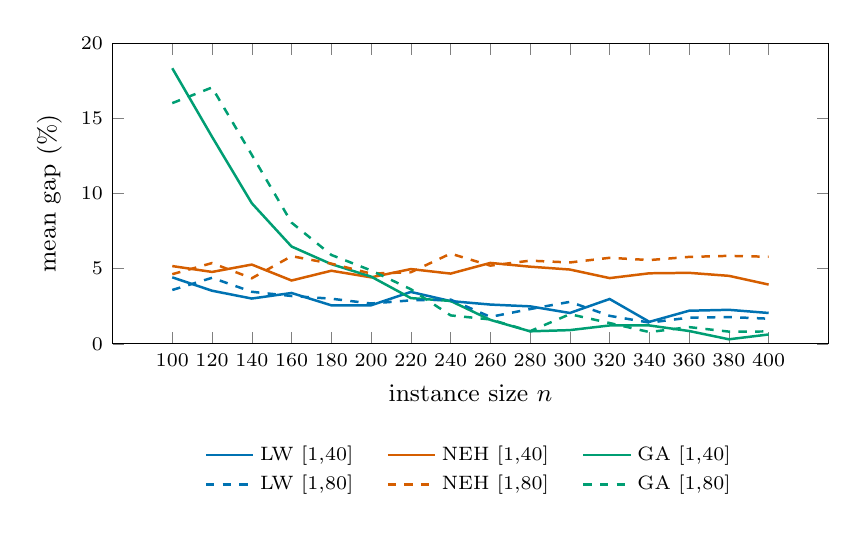
\begin{tikzpicture}
                \begin{axis}[
                    width=0.88\textwidth, height=5.4cm,
                    xlabel={instance size $n$}, ylabel={mean gap (\%)},
                    xtick={100,120,140,160,180,200,220,240,260,280,300,320,340,360,380,400}, xticklabels={100,120,140,160,180,200,220,240,260,280,300,320,340,360,380,400},
                    ymin=0, ymax=20,
                    tick label style={font=\scriptsize}, label style={font=\small},
                    every axis plot/.append style={line width=0.9pt},
                    legend columns=3,
                    legend style={font=\scriptsize, at={(0.5,-0.30)}, anchor=north, draw=none,
                        /tikz/every even column/.append style={column sep=10pt}},
                    ]
                    \addplot[apxblue] coordinates {(100,4.42) (120,3.53) (140,3.01) (160,3.38) (180,2.56) (200,2.56) (220,3.45) (240,2.84) (260,2.61) (280,2.49) (300,2.05) (320,2.98) (340,1.46) (360,2.20) (380,2.26) (400,2.05)};
                    \addlegendentry{LW $[1{,}40]$}
                    \addplot[nehred] coordinates {(100,5.17) (120,4.78) (140,5.27) (160,4.21) (180,4.86) (200,4.42) (220,4.97) (240,4.67) (260,5.38) (280,5.13) (300,4.94) (320,4.37) (340,4.69) (360,4.72) (380,4.52) (400,3.94)};
                    \addlegendentry{NEH $[1{,}40]$}
                    \addplot[gagreen] coordinates {(100,18.33) (120,13.77) (140,9.35) (160,6.47) (180,5.30) (200,4.47) (220,3.04) (240,2.85) (260,1.59) (280,0.83) (300,0.91) (320,1.22) (340,1.22) (360,0.85) (380,0.30) (400,0.62)};
                    \addlegendentry{GA $[1{,}40]$}
                    \addplot[apxblue, dashed] coordinates {(100,3.58) (120,4.39) (140,3.46) (160,3.18) (180,3.00) (200,2.68) (220,2.89) (240,2.94) (260,1.79) (280,2.31) (300,2.79) (320,1.86) (340,1.41) (360,1.74) (380,1.78) (400,1.67)};
                    \addlegendentry{LW $[1{,}80]$}
                    \addplot[nehred, dashed] coordinates {(100,4.63) (120,5.37) (140,4.36) (160,5.83) (180,5.33) (200,4.67) (220,4.76) (240,6.00) (260,5.20) (280,5.53) (300,5.41) (320,5.72) (340,5.57) (360,5.78) (380,5.85) (400,5.79)};
                    \addlegendentry{NEH $[1{,}80]$}
                    \addplot[gagreen, dashed] coordinates {(100,16.01) (120,17.05) (140,12.57) (160,8.06) (180,5.91) (200,4.88) (220,3.63) (240,1.89) (260,1.62) (280,0.84) (300,1.97) (320,1.38) (340,0.78) (360,1.11) (380,0.81) (400,0.82)};
                    \addlegendentry{GA $[1{,}80]$}
                \end{axis}
            \end{tikzpicture}
            \caption{Mean relative gap of the LW and the two heuristics on the large scale, against the lower bound $LB$. A solid line is $a_j,b_j\in[1,40]$, a dashed line $a_j,b_j\in[1,80]$.}
            \label{fig:gap-large}
        \end{figure}


        \section{Conclusion} \label{sec:conclusion}

        This paper studies the two-machine flow shop scheduling problem with the maximum weighted completion time objective.
        The problem is strongly NP-hard, and its optimal schedules exhibit a weight-based block structure, with Johnson's order within each block and blocks arranged in non-increasing order of weight.
        Exploiting this structure, we develop the $\mathbf{DP}$, an FPTAS for a fixed number of weight classes, and three heuristics  the $\mathbf{LW}$ rule, $\mathbf{NEH}$ and the $\mathbf{GA}$.

        Several directions for future research remain.
        First, the problem can be extended to more than two machines.
        Although the existing $\mathbf{MILP}$ formulation provides a starting point, the single-permutation property established for two machines does not generally hold for $m>2$.
        The extended model must therefore account for machine-specific sequencing decisions and precedence constraints between operations.
        Investigating the structural properties of optimal schedules in this setting may also provide a basis for developing more efficient exact and approximation algorithms.

        Second, for instances with more distinct weight classes, branch-and-bound offers a promising alternative to the $\mathbf{DP}$, whose computational requirements increase rapidly with $K$.
        The weight-based block structure can guide branching decisions, while the lower bounds can be used to evaluate partial schedules and prune unpromising nodes.
        Further improvements may be obtained by combining these bounds with dominance rules and heuristic solutions to establish strong upper bounds at early stages of the search.

        Third, the proposed heuristics can be extended to distributed flow shops, where job assignment to production shops and job sequencing must be optimized jointly.
        The $\mathbf{NEH}$ algorithm can be adapted to evaluate job insertions across candidate shops, accounting for both assignment and sequencing decisions.
        For the $\mathbf{GA}$, the chromosome can be extended to encode shop assignments together with job sequences, while the weight-block mutation can be retained or modified to preserve the structural advantages identified in this study.
        These extensions may provide effective solution approaches for larger and more complex production environments.

        \bibliographystyle{apalike}
        \bibliography{ref_IJPR}

    \end{sloppypar}
\end{document}

